\chapter{HeROfake : Orchestration serverless sur ressources hétérogènes pour le cloud privé}
\label{chapter:herofake}

% TODO: traduction française des figures

% TODO: détails sur la normalisation + scalarization~\cite{ehrgottMulticriteriaOptimization882005}

% TODO: détails sur Weighted Sum Method pour la résolution MOO + pourquoi pas ILP ? etc. + problème du front de Pareto avec WSM~\cite{marlerWeightedSumMethod2010} : comment choisir une solution plutôt qu'une autre ?

% TODO: phase hors-ligne : wattmètres logiciels comme PowerAPI~\cite{fieniPowerAPIPythonFramework2024}, EcoFloc~\cite{valeraEnergySavingPerspective}, Scaphandre et d'autres~\cite{jayExperimentalComparisonSoftwarebased2023}

% \section{Introduction}
% \label{section:herofake-introduction}

% \textbf{Modèle serverless}. Le serverless peut être compris à la fois comme un modèle de programmation, appelé Function as a Service (FaaS), et comme un modèle de déploiement pour le cloud. Dans un tel modèle, les développeurs conçoivent leurs applications comme une composition de fonctions sans état dont l'exécution est pilotée par des évènements~\cite{SchleierSmith2021WhatSC}. 
% Les services serverless libèrent les locataires d'une réservation complexe des ressources, car ils sont conçus pour gérer les exigences de mise à l'échelle à la demande.

% Dans le modèle FaaS, les fournisseurs ne facturent les clients qu'en fonction de leur utilisation réelle des ressources~\cite{jonasCloudProgrammingSimplified2019}. Ils sont entièrement responsables du déploiement d'une gestion intelligente des ressources et du multiplexage à une granularité plus fine afin d'optimiser les mesures de qualité de service (QoS) telles que le temps de réponse, la consommation d'énergie, etc.

\section{Introduction}
\label{section:herofake-introduction}

Dans le chapitre précédent, nous avons vu que certaines classes d'applications semblent particulièrement adaptées aux déploiements serverless. Pourtant, des défis entravent l'efficacité-coût du modèle et restent ouverts dans l'état de l'art. Dans ce chapitre, nous présentons notre première contribution, dans laquelle nous essayons d'apporter une réponse à la question suivante : 

\boitemagique{Question 1 (\textbf{QR1})}{
    Comment dimensionner les allocations dynamiques de ressources hétérogènes pour une application simple, constituée de fonctions sans dépendances, et comment ordonnancer efficacement les requêtes utilisateur, lorsque ces derniers ont des besoins variés en matière de qualité de service ?
}

Pour adresser les défis rencontrés par le fournisseur de services dans le cadre du déploiement d'applications dans le paradigme serverless, nous avons commencé par nous intéresser au cas d'applications simples, c'est-à-dire composées d'une unique fonction, et qui ne présentent donc pas de dépendances temporelles ou de données. En particulier, le cas des applications dites \textit{interactives} est intéressant : contrairement aux applications de traitements dits \textit{par lot}, les applications interactives présentent des motifs d'utilisation irréguliers, dépendant du comportement des utilisateurs, souvent difficile à anticiper ou à prédire avec précision~\cite{shahradServerlessWildCharacterizing, cncf2018whitepaper}. Ces applications sont sensibles à la latence, car leur exécution est dirigée par un évènement (une requête) ; toutefois, leurs utilisateurs peuvent avoir des exigences variées, et tolérer des écarts en matière de temps de réponse~\cite{buyyaSLAorientedResourceProvisioning2011}.

% \textbf{Détection de deepfake et serverless}.
Le travail présenté dans ce chapitre fait partie d'un projet (à l'institut de recherche b{\textless\textgreater}com \footnote{\href{https://b-com.com/fr/}{https://b-com.com/fr/}}) visant à déployer un service de détection de deepfake économe en énergie dans un cloud hétérogène. Les deepfakes sont des images, des vidéos ou des discours synthétiques, créés numériquement pour imiter une personne existante de manière à tromper leurs destinataires~\cite{westerlundEmergenceDeepfakeTechnology2019}. La détection de deepfake consiste à entraîner un réseau neuronal convolutif (CNN) pour détecter des motifs introduits lors du processus de génération.

% \boitemagique{Problème 1}{L'allocation de ressources au sein d'une plateforme serverless se fait sur un mode réactif, c'est-à-dire en réponse à une variation du trafic. Lorsque de nouvelles instances des fonctions doivent être déployées, cela provoque une latence additionnelle qui peut dégrader la qualité de service pour les utilisateurs. Le problème est particulièrement saillant dans l'environnement hautement hétérogène qu'est celui du cloud : les ressources matérielles ont différents niveaux de performances et de coût ; les applications interactives (c'est-à-dire dirigée par les évènements, par opposition à une application par lots) présentent des motifs d'usage difficilement prévisibles ; et les utilisateurs ont des besoins irréguliers et variés en qualité de service.}

% \textbf{Énoncé du problème}.
Le problème que nous tentons de résoudre dans ce chapitre est de déterminer comment dimensionner automatiquement et de manière réactive les allocations de ressources matérielles hétérogènes dans le cloud, en fonction de la charge sur l'application et des exigences de qualité de service des utilisateurs, tout en maintenant le coût des ressources et de l'énergie au niveau le plus bas possible pour le fournisseur.

\begin{table*}[!ht]
    \centering
    \caption{État de l'art des solutions de déploiement avec mise à l'échelle automatique pour des tâches de courte durée}
    \resizebox{\textwidth}{!}{
        \begin{tabular}{lccccccc}
            \toprule
            & Serverless & Target cloud platform     & SLA & Hardware heterogeneity & Resources usage & Energy consumption & Cost-aware \\
            \cmidrule(lr){2-2}\cmidrule(lr){3-3}\cmidrule(lr){4-4}\cmidrule(lr){5-5}\cmidrule(lr){6-6}\cmidrule(lr){7-7}\cmidrule(lr){8-8}
            Swayam~\cite{gujaratiSwayamDistributedAutoscaling2017}        & \xmark         & Private (Azure, in-house) & \cmark& \xmark                     & \cmark            & \xmark                 & \xmark         \\
            Pigeon~\cite{lingPigeonDynamicEfficient2019}                  & \cmark       & Private                   & \xmark  & \cmark                   & \cmark            & \xmark                 & \xmark         \\
            MArk~\cite{zhangMArkExploitingCloud}                          & \xmark         & Public (AWS)              & \cmark& \cmark                   & \cmark            & \xmark                 & \cmark       \\
            ENSURE~\cite{sureshENSUREEfficientScheduling2020}             & \cmark       & Private                   & \xmark  & \xmark                     & \cmark            & \xmark                 & \cmark       \\
            Mampage et al.~\cite{mampageDeadlineawareDynamicResource2021} & \cmark       & Private                   & \cmark& \xmark                     & \cmark            & \xmark                 & \cmark       \\
            Atoll~\cite{singhviAtollScalableLowLatency2021}               & \cmark       & Private                   & \cmark& \xmark                     & \xmark              & \xmark                 & \xmark         \\
            INFless~\cite{yangINFlessNativeServerless2022}                & \cmark       & Private                   & \cmark& \xmark                     & \cmark            & \xmark                 & \cmark       \\
            SMIF~\cite{choSLADrivenMLInference}                           & \cmark       & Private                   & \cmark& \cmark                   & \cmark            & \xmark                 & \xmark         \\
            Target solution                                                & \cmark       & Private                   & \cmark& \cmark                   & \cmark            & \cmark               & \cmark       \\ \bottomrule
        \end{tabular}
    }
    \label{table:herofake-sota}
\end{table*}

% \textbf{État de l'art}.
De précédentes études ont exploré le besoin d'une plateforme de mise à l'échelle automatique (ou \textit{autoscaling}) qui prend en charge les tâches de courte durée, à l'image de l'inférence. Le tableau~\ref{table:herofake-sota} résume les différences entre ces solutions et la plateforme cible que nous essayons de proposer ; la section~\ref{section:herofake-sota} rentre plus amplement dans le détail. Bien que de nombreuses contributions aient établi la nécessité de l'accélération à la demande pour garantir le temps de réponse des fonctions, aucune n'a mesuré l'impact de l'utilisation de ressources hétérogènes sur la consommation d'énergie dynamique. En outre, les études précédentes considèrent la consolidation des tâches comme un moyen de libérer des ressources pour d'autres calculs -- nous soutenons que ces techniques ouvrent des possibilités pour le fournisseur de services d'appliquer des politiques d'économie d'énergie dans le cloud privé. Enfin, comme les plateformes serverless sont des briques logicielles généralistes, conçues pour être hautement configurables, nous souhaitons proposer une solution basée sur les coûts, qui permette au fournisseur de faire des choix de configuration cohérents étant donnés ses objectifs d'optimisation.

% \textbf{Notre contribution}.
Nous soutenons qu'utiliser de manière opportuniste des accélérateurs matériels (GPU et FPGA) pour déployer des tâches de détection de deepfake peut permettre à un fournisseur de services cloud de garantir le temps de réponse des tâches et d'atteindre les SLA tout en réduisant l'utilisation des ressources et la consommation d'énergie. Dans ce chapitre, nous proposons \textbf{HeROfake} (pour \textit{\textbf{He}terogeneous \textbf{R}esources \textbf{O}rchestration for deep\textbf{fake} detection}), un framework complet pour déployer une application de détection de deepfake dans un cloud serverless. Ce framework comprend une phase hors-ligne et une phase en ligne. Durant la \textbf{phase hors-ligne}, nous caractérisons des plateformes matérielles hétérogènes et des tâches d'inférence en matière de performances et de consommation d'énergie. Durant la \textbf{phase en ligne}, notre orchestrateur se charge de passer automatiquement à l'échelle les fonctions déployées, et ordonnance les requêtes utilisateur de manière à utiliser efficacement les ressources matérielles à disposition pour atteindre les accords de niveau de service par requête, tout en réduisant la consommation d'énergie totale de la plateforme.

% Pour cette étude de cas, nous avons conçu un environnement de simulation qui modélise l'infrastructure cloud privée et l'application de détection de deepfake, déployée par le fournisseur sur une plateforme serverless.

% \textbf{Quelques mesures de performance}.
Avec notre politique d'allocation et d'ordonnancement, la plateforme est en mesure de traiter $50 000$ tâches dans le même laps de temps que Knative, avec moins de 36\% de pénalités de QoS. Notre stratégie réduit la consommation d'énergie dynamique pour l'exécution des tâches de près de 35\%, et permettrait au fournisseur de réduire davantage la consommation d'énergie statique en consolidant les tâches sur moins de 29\% des nœuds disponibles.

Ce chapitre est organisé comme suit : dans une première section~\ref{section:herofake-deepfake}, nous décrivons le modèle de plateforme global pour le projet. Dans la section~\ref{section:herofake-offline}, nous décrivons la phase hors-ligne de caractérisation des plateformes d'exécution et des tâches d'inférence. Dans la section~\ref{section:herofake-online}, nous rappelons les défis liés à l'orchestration dynamique de ressources hétérogènes lors de la phase en ligne, puis nous décrivons notre modèle de tâches et les politiques d'allocation et d'ordonnancement de l'orchestrateur. La section~\ref{section:herofake-evaluation} présente notre méthodologie d'évaluation et l'analyse des résultats expérimentaux. La section~\ref{section:herofake-sota} donne des détails concernant notre étude de l'état de l'art sur les plateformes d'autoscaling. Enfin, nous concluons dans la section~\ref{section:herofake-conclusion} et donnons quelques perspectives pour des travaux futurs.

\section{Motivation}
\label{section:herofake-motivation}

% Description de la charge de travail
Les fonctions utilisées par notre application de détection de deepfake répondent à trois caractéristiques principales typiques d'une charge de travail adaptée au modèle serverless~\cite{cncf2018whitepaper}. D'une part, la détection de deepfake à l'aide de réseaux de neurones convolutifs (CNN) est une tâche qui peut tirer parti de la concurrence par l'exécution de plusieurs convolutions en parallèle et/ou en traitant différentes images sur plusieurs cœurs de processeurs. Ces tâches sont dites sans état, car elles appliquent une transformation pure sur les données d'entrée -- en prenant une image en entrée et en renvoyant une valeur booléenne en sortie. Enfin, une telle application est dirigée par les évènements : le calcul est déclenché suite à l'envoi d'une image par l'utilisateur.
En outre, il serait coûteux de réserver à l'avance les ressources matérielles nécessaires pour exécuter cette application à l'échelle. Être en mesure de faire évoluer dynamiquement la quantité et la nature des ressources engagées en fonction de la demande permettrait à l'institut de réaliser d'importantes économies, en ne mobilisant pas plus de ressources que nécessaire pour cette application dans son infrastructure.

Pour ces raisons, nous pensons que le modèle de service serverless est adapté pour exécuter des tâches d'inférence à la demande avec un bon rapport coût-efficacité. Mais en raison de la nature éphémère des ressources non réservées, la latence, le débit et la continuité de service sont difficiles à garantir dans un contexte serverless~\cite{vaneykSPECRGCloud2018, dartoisCuckooOpportunisticMapReduce2019}. Lorsque les applications ne reçoivent pas de requêtes entrantes, les environnements d'exécution des fonctions sont détruits au lieu d'être maintenus dans un état inactif. Lorsqu'une nouvelle requête arrive, le fournisseur doit (ré)allouer des ressources et initialiser les fonctions à nouveau : c'est ce que l'on appelle un démarrage à froid (ou \textit{cold start}). Les temps de démarrage à froid sont très préjudiciables aux performances de l'application. Dans certains cas, ils peuvent même dominer le temps d'exécution total d'une fonction~\cite{mullerLambadaInteractiveData2020}.

%\textbf{Hétérogénéité matérielle dans le cloud}.
Les infrastructures cloud sont de plus en plus hétérogènes pour répondre aux besoins d'applications très consommatrices, telles que l'apprentissage machine ou l'analyse de données en masse~\cite{reissHeterogeneityDynamicityClouds}. Les travaux de l'état de l'art montrent que l'utilisation de ce type de matériel dans le cloud permet des gains substantiels en termes de temps d'exécution et de consommation d'énergie~\cite{10.1145/3369583.3392679, 9195730}. Cependant, les plateformes d'exécution spécialisées (telles que les GPU) ne sont pas disponibles dans les offres serverless commerciales~\cite{khandelwalTaureauDeconstructingServerless2020}, et les orchestrateurs open source de référence tels que Kubernetes avec Knative ou OpenWhisk ne prennent pas en charge l'allocation dynamique de ce type de matériel.

De plus, dans les offres commerciales serverless actuelles, les accords de niveau de service (SLA, pour \textit{Service Level Agreement}) sont généralement limités à garantir le traitement d'une requête (avec des redémarrages en cas d'échec), sans considérer son temps de réponse. De ce point de vue, l'absence de garanties de qualité de service dans les offres commerciales serverless limite l'utilité du modèle pour des cas d'usage critiques~\cite{buyyaSLAorientedResourceProvisioning2011}.

\section{Déployer des tâches de détection de deepfake dans un cloud serverless}
\label{section:herofake-deepfake}

Cette section présente le modèle de la plateforme serverless considérée, ainsi que le projet global dans lequel ces travaux s'inscrivent.

\subsection{Modèle de la plateforme}

\begin{figure*}[!ht]
    \centering
    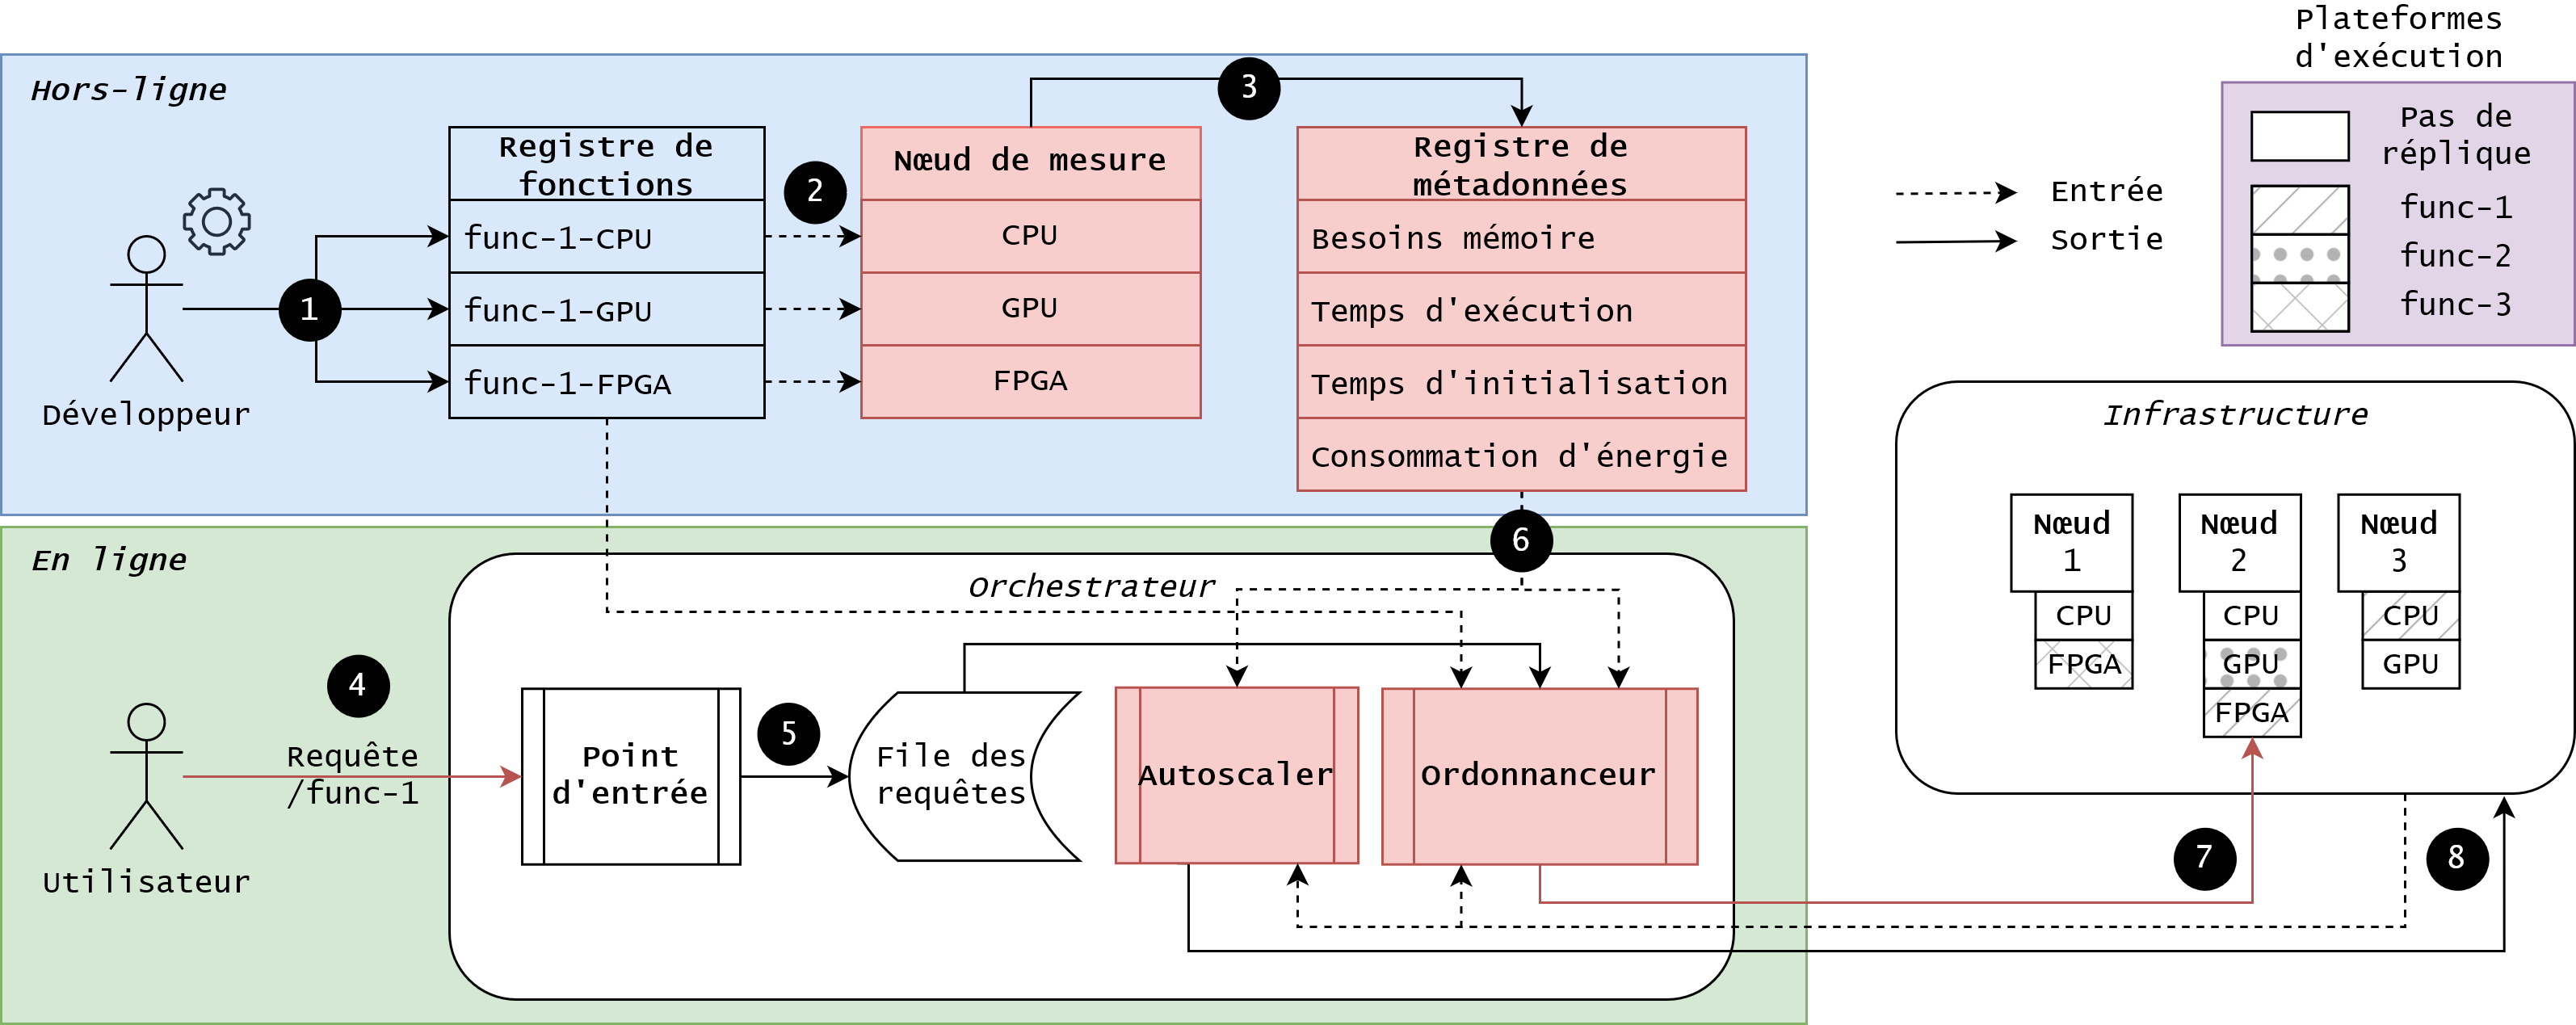
\includegraphics[width=0.8\textwidth]{4_Chapitre4/figures/placement.png}
    \caption{Plateforme serverless pour le déploiement d'une application de détection de deepfake ; vue d'ensemble du système.}
    \label{figure:herofake-placement}
\end{figure*}

Nous considérons un système de détection de deepfake, déployé comme une application serverless, composé de trois fonctions sans état qui réalisent des tâches d'inférence sur des images en entrée. Ces images sont toutes RGB et de taille $224 \cdot 224$ pixels. Les vidéos ne sont pas encore prises en compte à ce stade du projet.

La figure~\ref{figure:herofake-placement} présente la plateforme utilisée. Nous distinguons une phase \textit{hors-ligne} (boîte bleue dans la figure) et une phase \textit{en ligne} (boîte verte dans la figure). Pendant la phase hors-ligne, un nœud de mesure collecte les métadonnées relatives à l'exécution des tâches sur des plateformes d'exécution hétérogènes ; pendant la phase en ligne, un orchestrateur alloue les ressources matérielles nécessaires et ordonnance les requêtes utilisateur.

Les demandes d'invocation de fonctions (requêtes) émanant des utilisateurs sont reçues par le fournisseur et traitées par l'orchestrateur. Dans notre modèle, une invocation de fonction correspond à un \textit{tâche}. L'utilisateur sélectionne l'un des trois modèles fournis (ResNet50, VGG16 et VGG19 (voir section~\ref{section:herofake-offline:workload}) qui est utilisé pour détecter un éventuel deepfake.

L'infrastructure du fournisseur de cloud est modélisée comme un ensemble de \textit{nœuds} hétérogènes (section~\ref{model:nodes}) comprenant diverses combinaisons de \textit{plateformes} (section~\ref{model:platforms}) qui peuvent exécuter des \textit{tâches} pour traiter les requêtes entrantes (section~\ref{model:tasks}).

\subsubsection{Nœuds}
\label{model:nodes}

Un nœud est un serveur disponible dans l'infrastructure du fournisseur de services. Dans ce travail, nous ne tenons pas compte de la localité du stockage et des données. Les données d'entrée sont toujours fournies \textit{via} le téléchargement de fichiers par l'utilisateur au moment de sa requête. Nous considérons une durée uniforme pour ce téléchargement, qui est incluse dans le temps d'exécution total de la fonction. Ainsi, la seule caractéristique qui définit un nœud dans notre modèle d'infrastructure est la taille de la mémoire dédiée. Un nœud est constitué d'un ensemble de plateformes d'exécution définies ci-après.

\subsubsection{Plateformes d'exécution}
\label{model:platforms}

Une plateforme d'exécution est une unité de traitement matérielle disponible sur un nœud. Chaque plateforme consomme une quantité d'énergie à l'état "inactif" (\textit{idle}), exprimée en kilowattheures (kWh). Lorsqu'elle commence à exécuter une tâche, elle consomme une énergie supplémentaire caractérisée par les propriétés (le \textit{type}) de la tâche : la plateforme est alors dans un état "actif". Nous distinguons le temps "inactif" et le temps "actif" pour chaque plateforme, afin de mesurer l'utilisation des ressources. Les plateformes sont caractérisées par un \textit{type de plateforme} qui englobe les paramètres suivants :

\begin{itemize}
    \item \textit{Type de matériel} -- CPU, GPU ou FPGA ;
    \item \textit{Prix} -- le coût d'acquisition d'une telle plateforme par le fournisseur de services cloud ;
    \item \textit{Énergie au repos} -- la consommation d'énergie de base de la plateforme lorsqu'elle n'exécute aucune tâche.
\end{itemize}

\textbf{Mise en cache des tâches et modèle de démarrage à froid}. Nous considérons un mécanisme simple de mise en cache des tâches au niveau de la plateforme, qui s'apparente à un mécanisme de maintien en activité (\textit{keep-alive})~\cite{7279063}. Dans notre système, si une plateforme a déjà exécuté une tâche de type $t$ et qu'une nouvelle tâche du même type $t$ est programmée sur cette même plateforme, le délai de démarrage à froid n'est pas appliqué. Toutefois, si cette même plateforme devait exécuter une tâche de type différent $tt$, la tâche subirait un délai de démarrage à froid avant d'entrer dans sa phase d'exécution. Enfin, si la plateforme n'a pas été allouée précédemment, la tâche subira également un délai de démarrage à froid.

\subsection{Description générale du système}

L'institut de recherche b{\textless\textgreater}com travaille sur un projet qui vise à déployer une application de détection de deepfake sur un cloud privé. Les utilisateurs soumettent une image au système et lorsque leur requête est satisfaite, ils obtiennent une valeur booléenne en réponse. L'application vise différentes catégories d'utilisateurs : certains d'entre eux peuvent être des médias ou des autorités ayant des exigences élevées en matière de qualité de service, tandis que d'autres peuvent être des utilisateurs occasionnels tolérant une latence plus élevée.

Pour différencier ces catégories d'utilisateurs, nous proposons différents niveaux d'accords de niveau de service, applicables à la granularité d'une requête. Les utilisateurs ayant des exigences plus élevées accepteront de payer un prix plus élevé par requête, mais si nous ne parvenons pas à satisfaire leur requête dans le temps de réponse imparti, nous consentirons à une remise -- plus le niveau de qualité de service est élevé, plus la remise est importante. Le fournisseur est donc fortement incité, sur le plan financier, à garantir la qualité de service.

\textbf{Phase hors-ligne}. Dans notre plateforme, le cycle de vie de l'application commence par une phase hors-ligne au cours de laquelle le développeur fournit le code de ses fonctions pour différentes architectures matérielles \Circled{1}. Ce code est stocké dans un registre de fonctions. Les fonctions sont ensuite déployées sur un nœud de mesure \Circled{2} où elles sont exécutées afin de générer des métadonnées relatives aux fonctions : les besoins en mémoire, le temps d'exécution, le temps de démarrage à froid et la consommation d'énergie pour chaque fonction sont écrits dans un registre de métadonnées \Circled{3}. La phase hors-ligne doit être exécutée une fois pour une fonction donnée sur une plateforme donnée, elle est décrite dans la section~\ref{section:herofake-offline}.

\textbf{Phase en ligne}. Lorsqu'un utilisateur envoie une requête à l'application \Circled{4}, il fournit une image d'entrée et spécifie le niveau de qualité de service souhaité. La requête est ajoutée à une file d'attente \Circled{5} au niveau de l'orchestrateur. Lorsque l'ordonnanceur extrait la requête de la file d'attente, le registre de métadonnées est interrogé pour récupérer les métadonnées de fonction appropriées \Circled{6}.

L'\textbf{ordonnanceur} tente ensuite de planifier une tâche (c'est-à-dire l'invocation d'une fonction) pour répondre à la requête. Les tâches sont placées sur des \textit{répliques} de fonctions \Circled{7} déjà déployées. Ces répliques peuvent être des conteneurs ou des machines virtuelles, c'est-à-dire des environnements d'exécution dédiés pour la fonction donnée. Simultanément, l'\textbf{autoscaler} surveille les files d'attente de requêtes dans toutes les répliques de fonctions \Circled{8}. Le rôle de l'autoscaler est de dimensionner les ressources allouées en fonction des fluctuations de charge pour chaque fonction. L'ordonnanceur et l'autoscaler sont décrits dans la section~\ref{section:herofake-online}.

\section{Phase hors-ligne : mesures et extraction des métadonnées}
\label{section:herofake-offline}

\subsection{Caractérisation des plateformes d'exécution}

\begin{table}[!ht]
    \caption{Execution platform characterization}
    \begin{center}
    \resizebox{\columnwidth}{!}{%
    \begin{tabular}{|c|c|c|c|c|}
    \hline
                                 \textbf{Platform} & \textbf{Hardware type}& \textbf{Price (MSRP)} & \textbf{Idle energy} \\ \hline
    Intel Xeon ES-1620 v4         & CPU           & 294          & 0.067       \\ \hline
    Nvidia GeForce RTX 2070 Super & GPU           & 499          & 0.010       \\ \hline
    Xilinx Alveo U250             & FPGA          & 7695         & 0.030       \\ \hline
    \end{tabular}%
    }
    \end{center}
    \label{table:herofake-platforms}
\end{table}

La demande grandissante pour l'apprentissage machine et l'inférence, ainsi que l'augmentation de la consommation d'énergie dans le cloud~\cite{masanetRecalibratingGlobalData2020}, font de l'efficacité énergétique des dispositifs cibles devient une préoccupation majeure. Les accélérateurs basées sur les FPGA sont décrits comme un concurrent pertinent à l'hégémonie des GPU. Nous proposons un benchmark de l'efficacité énergétique de plusieurs plateformes matérielles (CPU, GPU, FPGA) pendant la phase d'inférence pour plusieurs réseaux neuronaux convolutifs (CNN) utilisés dans le framework de la détection de deepfake. Notre comparaison porte sur des métriques de consommation d'énergie, de vitesse d'inférence et de précision. Ces mesures sont cruciales pour une orchestration efficace sur des plateformes hétérogènes.

Le CPU caractérisé est un Intel Xeon CPU ES-1620 v4 (3,5 GHz) ; le GPU est une Nvidia GeForce RTX 2070 Super. Ces deux modèles sont compatibles avec les versions récentes de TensorFlow, une des plateformes principales utilisées pour l'inférence. Si les procédés de fabrication pour ces deux accélérateurs sont comparables, la finesse de gravure à 12 nm pour le GPU contre 16 nm pour le FPGA pourrait donner un léger avantage au GPU dans ce benchmark.

En ce qui concerne le FPGA, nous avons utilisé l'Alveo U250, une carte dédiée au cloud et fabriquée par Xilinx. Ce FPGA est compatible avec Vitis-AI~\cite{vitis-ai}, que nous avons utilisé pour exécuter les tâches d'inférence sur le FPGA. Nous avons utilisé la dernière version disponible (v. 2.0) au moment de cette étude. Vitis-AI propose deux méthodes pour l'optimisation des modèles, nécessaire à leur exploitation sur un FPGA limité en ressources mémoire. La première est l'élagage, qui consiste à réduire la complexité du modèle par une compression tout en supprimant certaines sections non critiques de l'arbre. La seconde est la quantification, qui consiste à convertir les poids flottants de 32 bits en entiers de 8 bits. Nous avons utilisé cette dernière méthode pour optimiser notre modèle avant la compilation, qui convertit notre modèle en instructions DPU (\textit{Deep Processing Unit}).

\subsection{Caractérisation des tâches logicielles}
\label{section:herofake-offline:workload}

\begin{table}[!ht]
    \caption{Workload characterization}
    \centering
    \resizebox{\columnwidth}{!}{%
    \begin{tabular}{|c|cc|ccc|ccc|ccc|}
    \hline
    Task     & \multicolumn{2}{c|}{Memory (GB)} & \multicolumn{3}{c|}{Cold start (s)}                              & \multicolumn{3}{c|}{Execution time (s)}                         & \multicolumn{3}{c|}{Energy (mWh)}                            \\ \hline
             & \multicolumn{1}{c|}{CPU}  & GPU  & \multicolumn{1}{c|}{CPU}   & \multicolumn{1}{c|}{GPU}   & FPGA   & \multicolumn{1}{c|}{CPU}   & \multicolumn{1}{c|}{GPU}   & FPGA  & \multicolumn{1}{c|}{CPU}  & \multicolumn{1}{c|}{GPU}  & FPGA \\ \hline
    ResNet50 & \multicolumn{1}{c|}{1.3}  & 3.3  & \multicolumn{1}{c|}{1.232} & \multicolumn{1}{c|}{2.340} & 9.952  & \multicolumn{1}{c|}{0.124} & \multicolumn{1}{c|}{0.024} & 0.009 & \multicolumn{1}{c|}{3.11} & \multicolumn{1}{c|}{1.7}  & 0.5  \\ \hline
    VGG16    & \multicolumn{1}{c|}{1.8}  & 3.3  & \multicolumn{1}{c|}{2.514} & \multicolumn{1}{c|}{4.641} & 14.528 & \multicolumn{1}{c|}{0.143} & \multicolumn{1}{c|}{0.046} & 0.010 & \multicolumn{1}{c|}{4.34} & \multicolumn{1}{c|}{3.43} & 0.55 \\ \hline
    VGG19    & \multicolumn{1}{c|}{1.9}  & 3.4  & \multicolumn{1}{c|}{2.559} & \multicolumn{1}{c|}{4.641} & 14.758 & \multicolumn{1}{c|}{0.167} & \multicolumn{1}{c|}{0.048} & 0.012 & \multicolumn{1}{c|}{5.16} & \multicolumn{1}{c|}{3.58} & 0.65 \\ \hline
    \end{tabular}
    }%
    \label{table:herofake-tasks}
\end{table}

Nous avons caractérisé trois modèles populaires au moment de cette étude. Le premier, ResNet50, est basé sur les réseaux neuronaux résiduels. Il utilise des blocs résiduels et peut être entraîné efficacement~\cite{NEURIPS2019_7716d0fc}. Le second est VGG16 (VGG pour \text{Visual Geometry Group}), qui utilise uniquement des convolutions comme blocs~\cite{DBLP:journals/corr/SimonyanZ14a} et le troisième est VGG19, une variante de VGG16 avec trois couches supplémentaires~\cite{biom10070984}. Ces réseaux sont entraînés sur un GPU, l'entraînement n'étant pas le sujet de cette étude.

\subsection{Mesures de performances}

\begin{figure}[!ht]
    \centering
    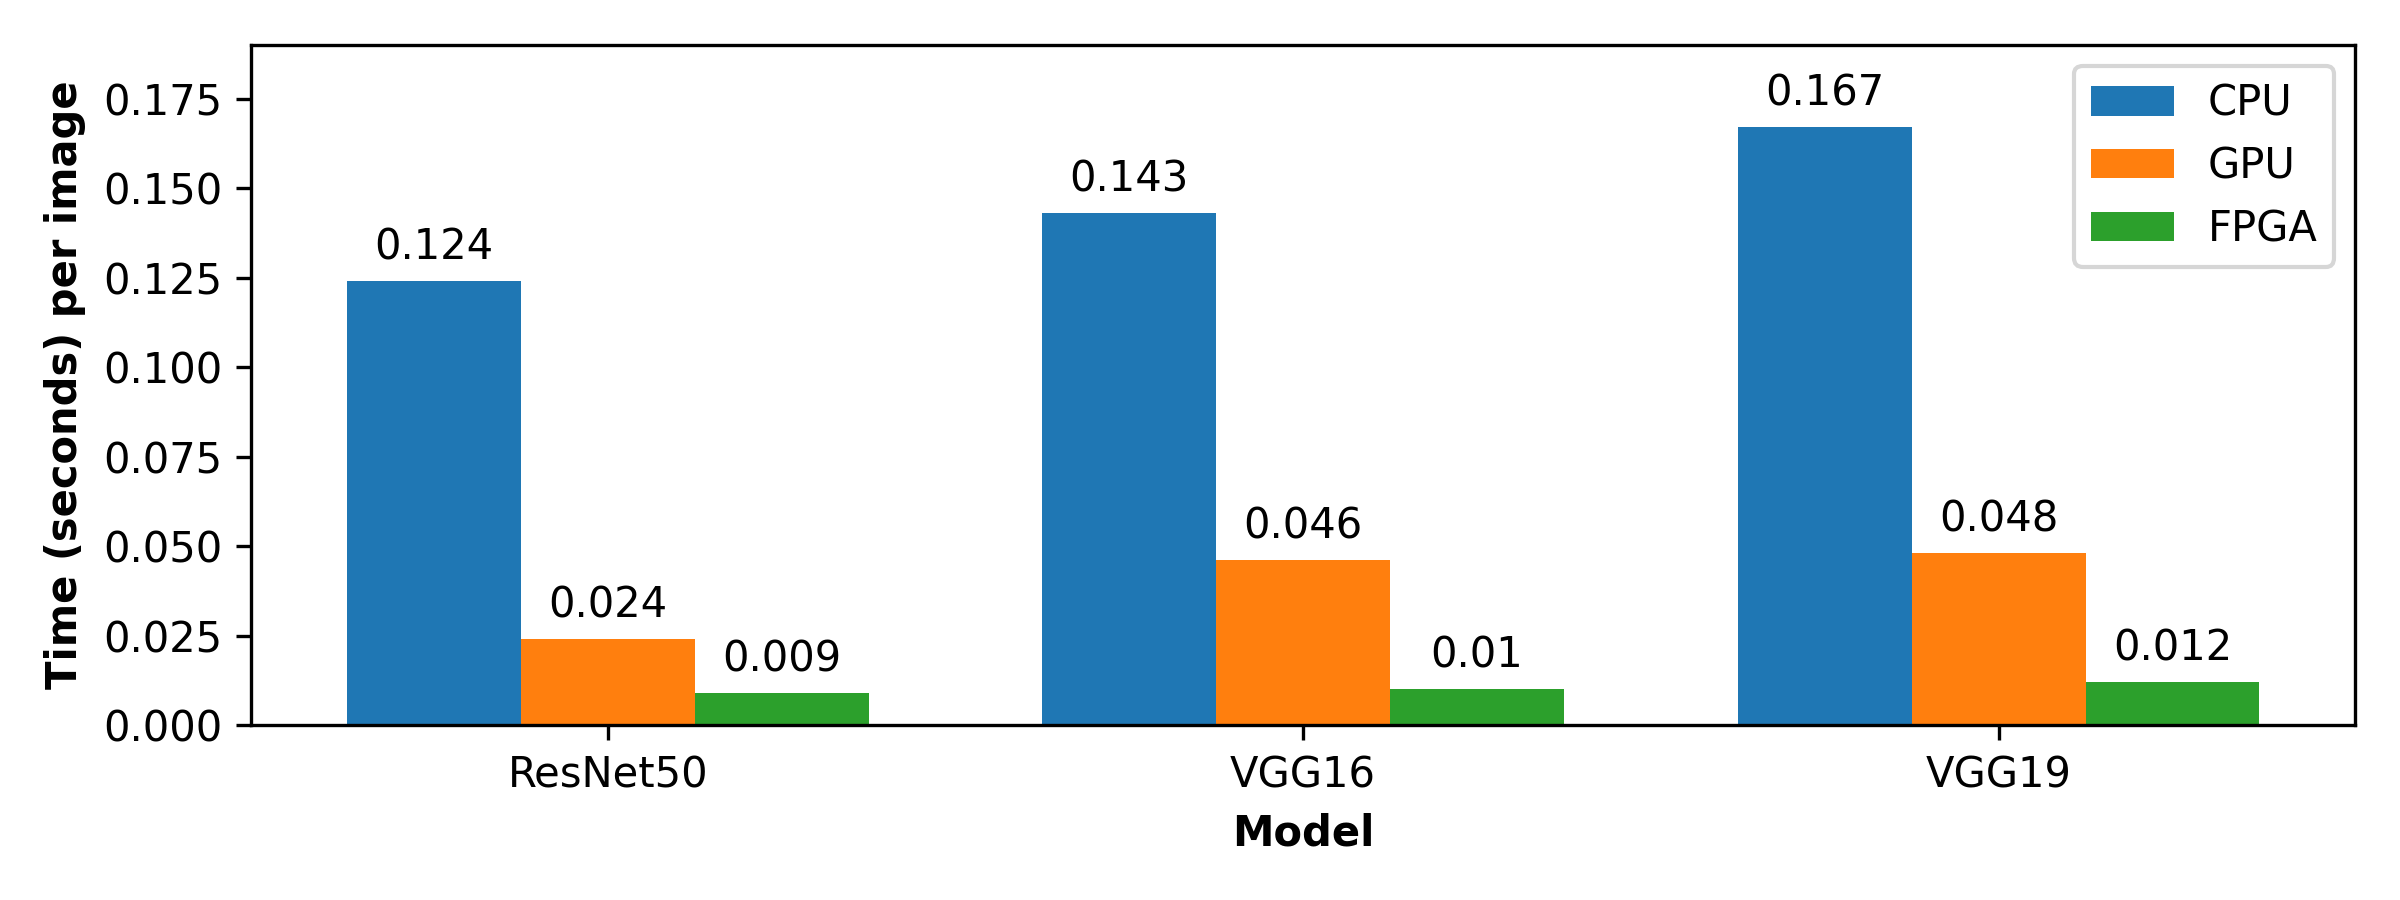
\includegraphics[width=\columnwidth]{4_Chapitre4/figures/characterization/time_of_inference_1_image.png}
    \caption{Inference time for one image with ResNet50, VGG16 and VGG19.}
    \label{figure:herofake-time-inference}
\end{figure}

La carte d'accélération FPGA étant censée être plus efficace qu'un CPU ou un GPU~\cite{5272532}, la comparaison du temps d'inférence avec ces trois technologies est une première condition pour permettre la comparaison du coût énergétique par image. L'évaluation des performances en termes de temps d'exécution a été réalisée avec les mêmes 10000 images pour les trois modèles différents. Nous avons construit un jeu de données à deux classes : d'une part, de vraies images provenant du jeu de données CelebA~\cite{https://doi.org/10.48550/arxiv.1411.7766}, et d'autres part des images synthétiques générées à l'aide d'un \textit{Generative Adversarial Network} (GAN)~\cite{jimaging7080128}. La quantification et la compilation du modèle ont été effectuées avec Vitis-AI afin de l'exécuter sur le FPGA. En ne considérant que le temps d'inférence, il s'est avéré que sur les trois modèles testés (ResNet50, VGG16 et VGG19), le FPGA est de 13,08 à 13,79 fois plus rapide que le CPU mais aussi de 2,52 à 4,48 fois plus rapide que le GPU (voir figure~\ref{figure:herofake-time-inference}).

\subsection{Mesures de consommation d'énergie}

\begin{figure}[!ht]
    \centering
    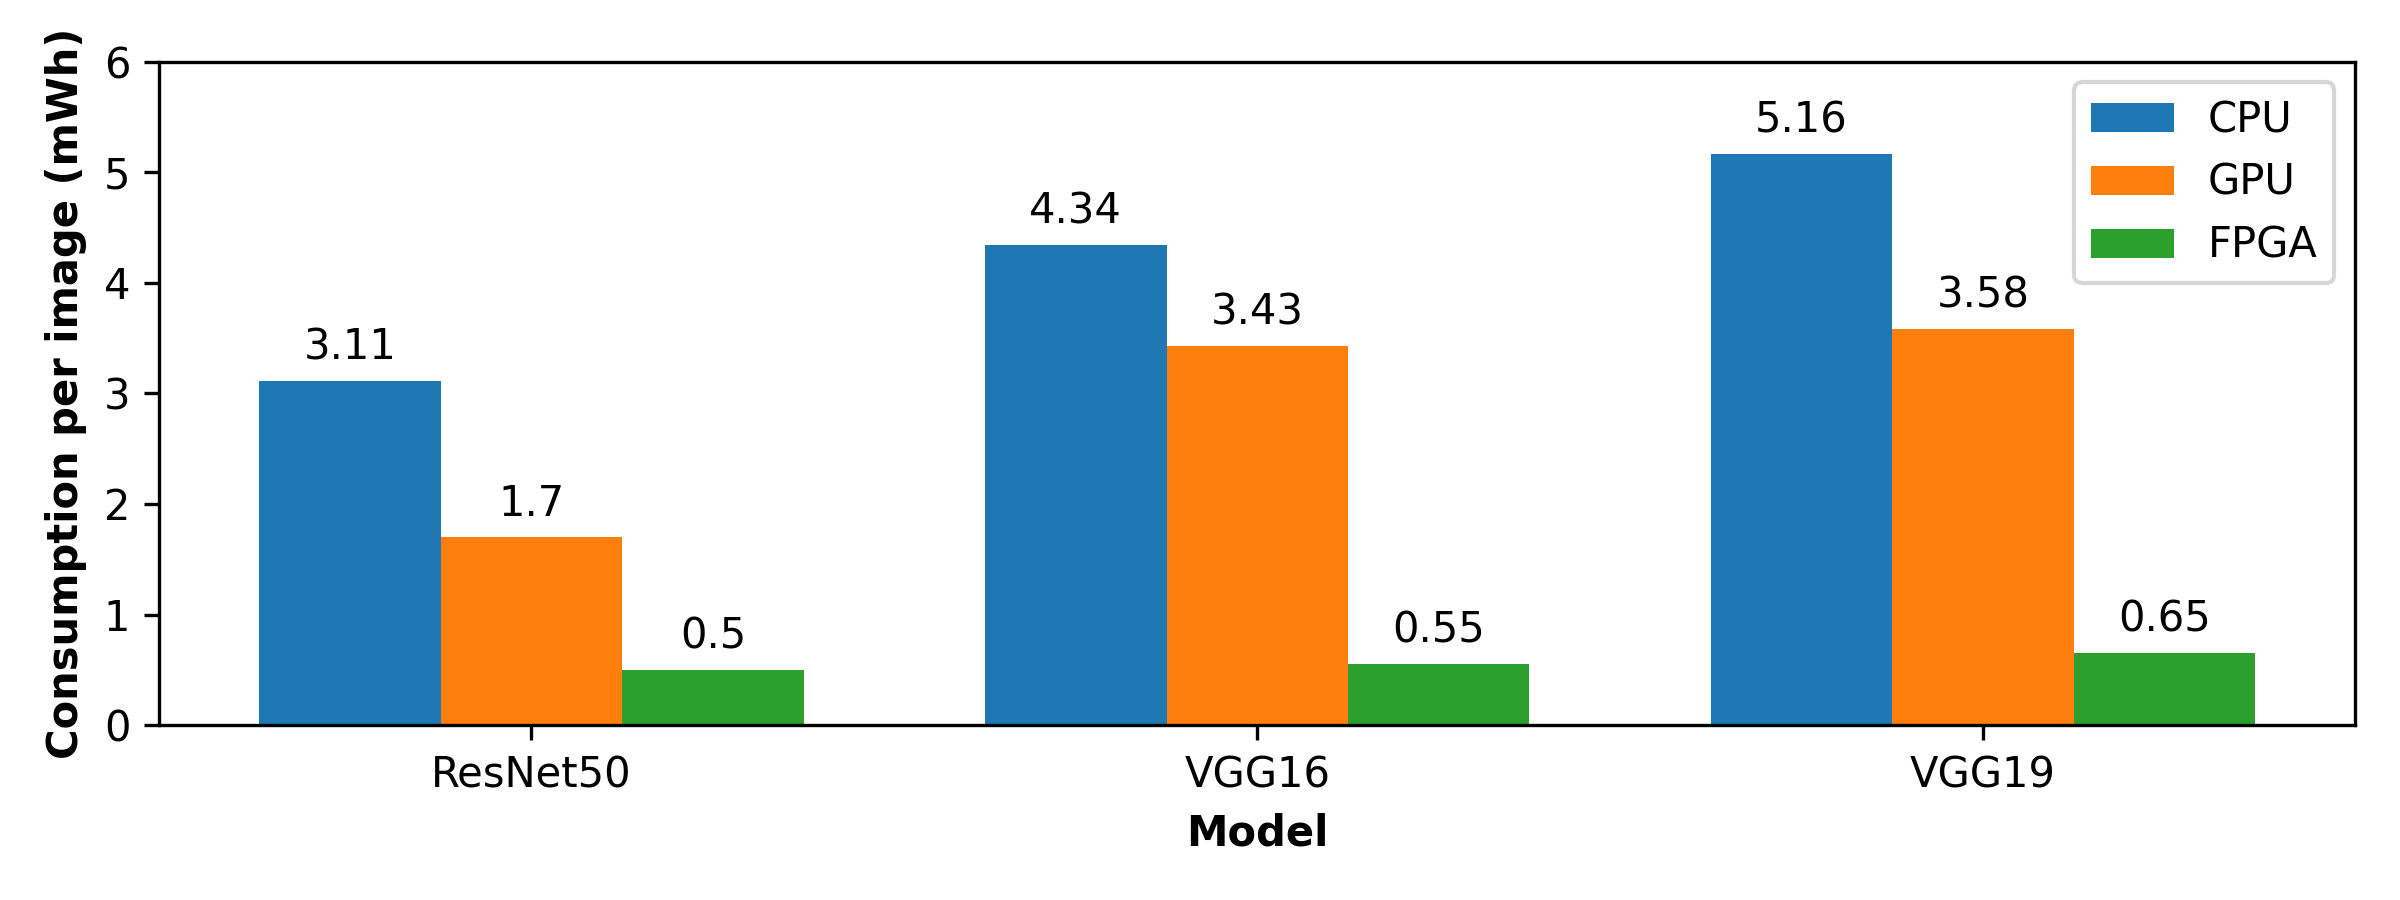
\includegraphics[width=\columnwidth]{4_Chapitre4/figures/characterization/consumption_per_image.png}
    \caption{Energy consumption of inference per image (mWh).}
    \label{figure:herofake-consumption-per-image}
\end{figure}

La consommation d'énergie instantanée mesurée pendant l'inférence correspond à la consommation globale de la machine (y compris le CPU, la mémoire, la carte mère et l'alimentation) pendant l'exécution de l'inférence.
Les mesures ont été effectuées à l'aide d'une alimentation spécifique (PDU pour \textit{Power Distribution Unit}), en l'occurrence une Raritan PX3-5190R, capable de surveiller la puissance instantanée et la consommation d'énergie du serveur (Dell Precision T5810). Les résultats montrent que l'inférence sur le CPU produit la consommation d'énergie instantanée la plus faible. Ce résultat est assez attendu car l'inférence sur GPU ou FPGA induit également une consommation d'énergie par le CPU.

Cependant, la seule consommation d'énergie instantanée ne reflète pas correctement le coût total de chaque plateforme. Le temps d'exécution nécessaire pour traiter toutes les images doit être pris en compte. La mesure pertinente est le coût énergétique par image. La consommation d'énergie a été mesurée en kilowattheures (kWh) pour les 10000 images, puis convertie en milliwattheures (mWh) par image. De ce point de vue, il est clair que le FPGA est le plus économe en énergie étant donné le temps d'exécution : sa consommation est de 6,2 à 6,9 fois moindre que pour le CPU, et de 3,3 à 6,2 fois moindre que pour le GPU (voir figure~\ref{figure:herofake-consumption-per-image}).

\subsection{Discussion}

\begin{figure}[!ht]
    \centering
    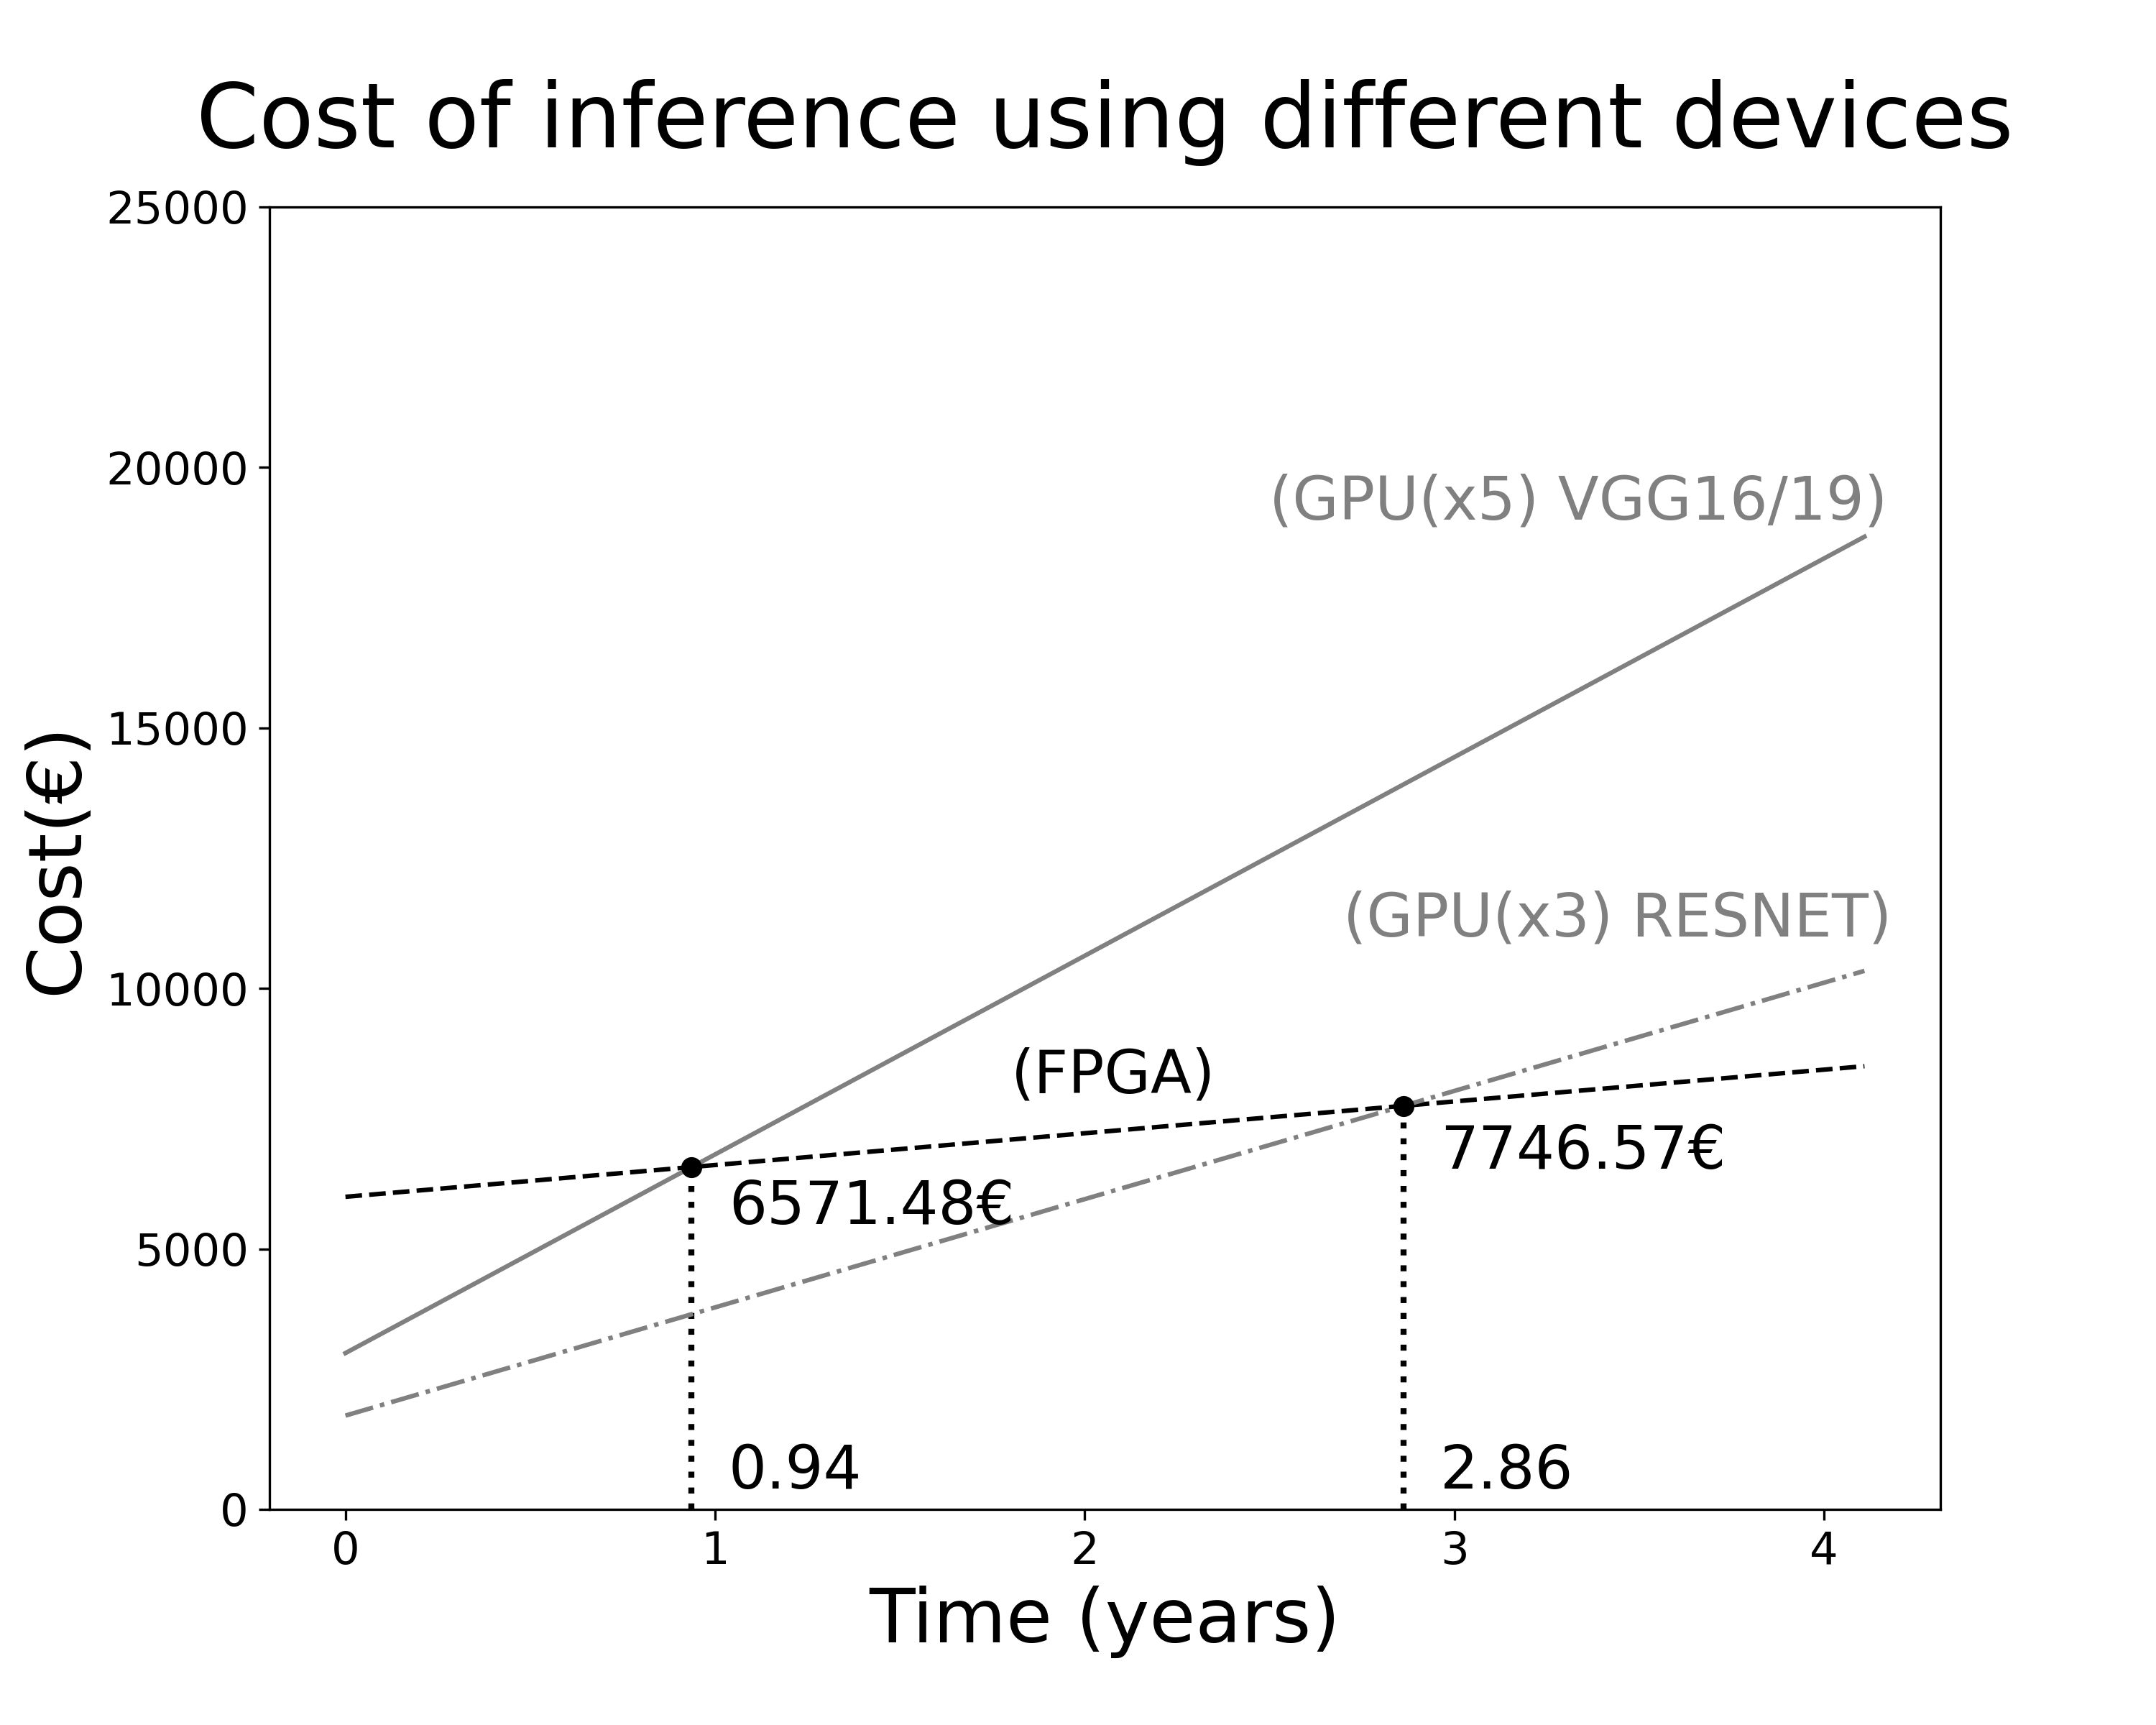
\includegraphics[width=\textwidth]{4_Chapitre4/figures/characterization/cost_devices_time.png}
    \caption{Total cost of inference on selected devices over time.}
    \label{figure:herofake-cost-over-time}
\end{figure}

Les résultats de ce benchmark montrent un net avantage en faveur du FPGA pour l'inférence en termes de performance et d'efficacité énergétique. Les gains de performance sont significatifs, en particulier avec les réseaux d'apprentissage profond plus complexes~\cite{8782524}. % Les ressources informatiques basées sur des serveurs équipés de cartes d'accélération FPGA, au lieu de cartes d'accélération GPU, bénéficieraient de ces avantages.

Cependant, la consommation d'énergie brute du dispositif ne reflète pas le coût total de la solution. En effet, il faut également inclure le coût de l'équipement lui-même. C'est un point important dans la comparaison entre GPU et FPGA, car il existe un écart de prix important entre les deux technologies : le GPU (RTX 2070 Super) utilisé pour ce benchmark a été lancé aux alentours de 600€, alors que le FPGA (Alveo U250) est vendu aux alentours de 6000€. En Europe, le coût de l'électricité pour effectuer l'inférence est très faible (nous avons utilisé la moyenne européenne de 0,1833€ par kWh au moment de cette étude~\cite{energy-price}), comparé au coût initial du dispositif : la durée d'exécution nécessaire pour bénéficier de l'avantage-coût du FPGA est de l'ordre de plusieurs mois de fonctionnement continu. La figure~\ref{figure:herofake-cost-over-time} représente le coût cumulé (en euros) de l'utilisation d'un serveur avec accélération GPU ou FPGA en fonction du temps (en années). Notre estimation du coût comprend le nombre de GPU nécessaires et leur coût pour rivaliser avec les performances des FPGA, et est pondérée d'un facteur 2x~\cite{shehabiUnitedStatesData2016} pour tenir compte de la consommation d'énergie totale de l'infrastructure (principalement le refroidissement et les équipements réseau). Le FPGA peut devenir une solution rentable après quelques mois pour les CNN complexes. Pour les réseaux moins complexes, l'avantage financier du FPGA est atteint après plus de deux ans.

\begin{figure}[!ht]
    \centering
    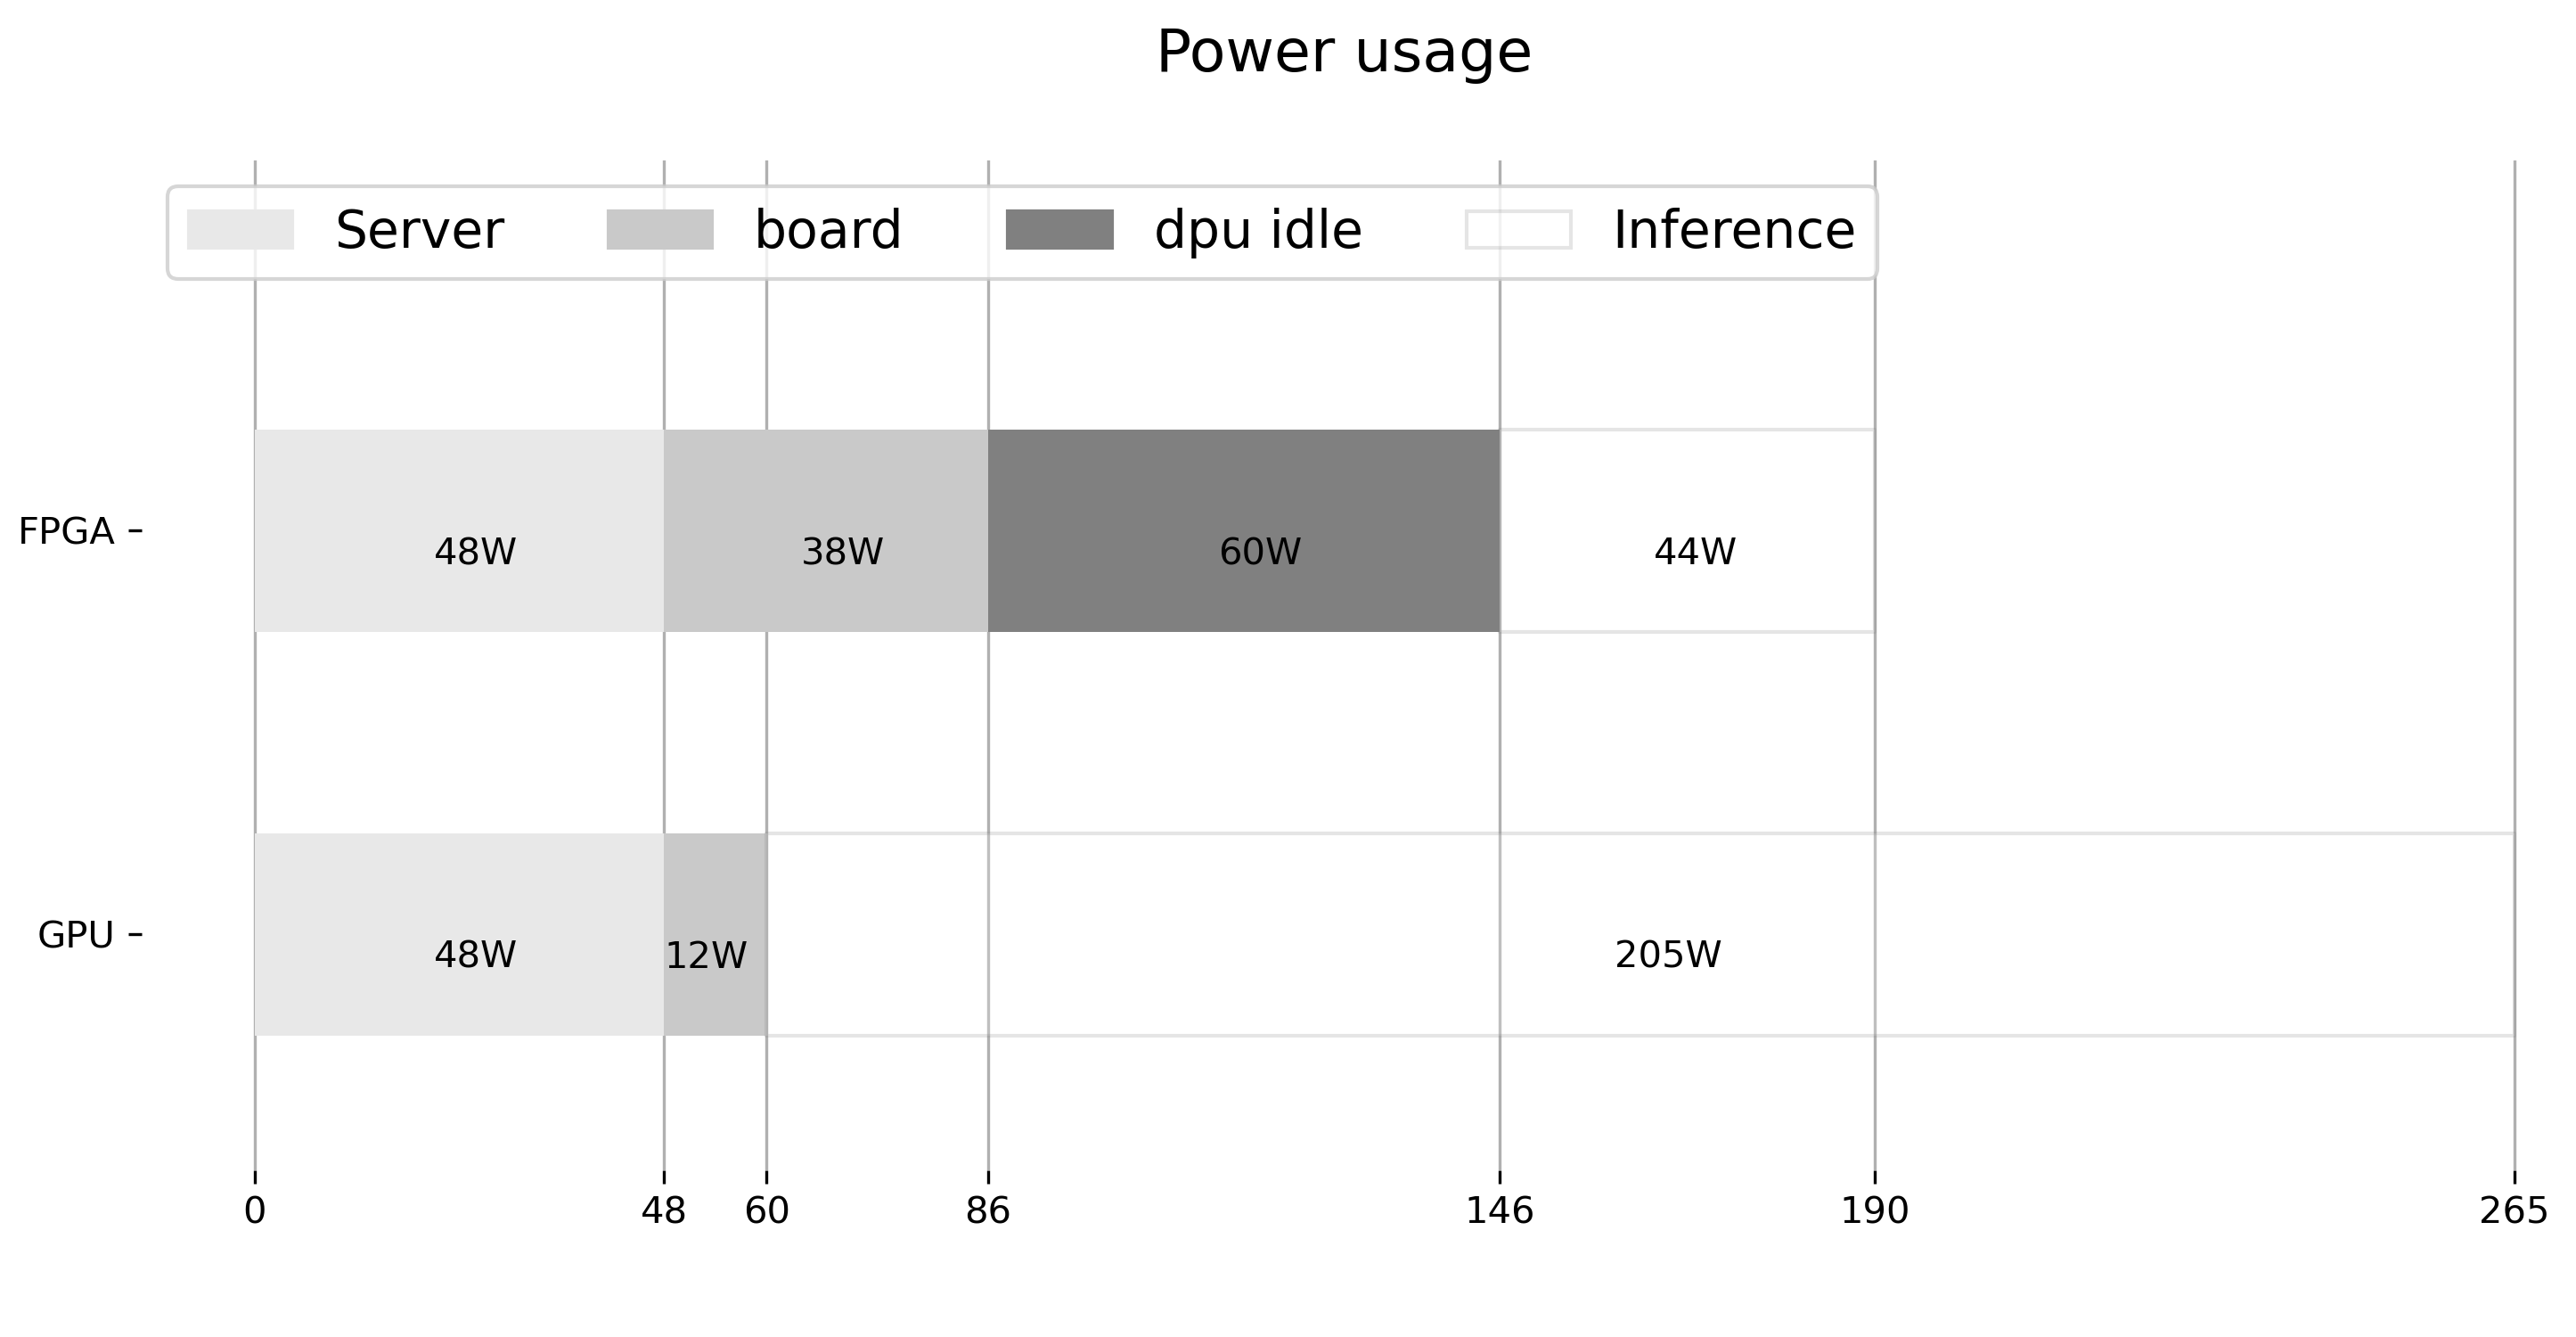
\includegraphics[width=\columnwidth]{4_Chapitre4/figures/characterization/power_usage.png}
    \caption{Power usage breakdown for FPGA and GPU.}
    \label{figure:herofake-power-usage}
\end{figure}

L'analyse précédente est valable dans le cas où l'inférence est toujours effectuée à pleine charge. En effet, lorsque l'on décompose la consommation d'énergie du GPU entre sa consommation au repos et sa consommation lors de l'inférence, il est clair que le GPU est capable d'adapter dynamiquement sa consommation d'énergie en fonction de l'intensité du traitement. Le FPGA, quant à lui, semble avoir une gestion de l'énergie très limitée. Une fois le modèle (\textit{DPU}, pour \textit{Deep Learning Processor Unit}) chargé dans le FPGA, la consommation d'énergie au repos est mesurée à un niveau élevé (figure~\ref{figure:herofake-power-usage}). En plus des 38W consommés au repos par la carte FPGA, on observe une consommation résiduelle de 60W, même lorsque le dispositif est inactif. Si des évolutions en matière d'implémentation du DPU sur le FPGA peuvent limiter l'impact de ce problème (par exemple en réduisant la fréquence d'horloge lorsqu'il est inactif), son influence sur le coût total doit être pris en compte si le dispositif n'est pas toujours utilisé à pleine charge. Avec seulement 12W d'énergie au repos, le GPU est un meilleur candidat lorsque l'utilisation à pleine charge du dispositif n'est pas garantie.

Comme la tendance vers des CNN plus complexes se poursuit~\cite{8807741}, l'utilisation de dispositifs les plus efficaces possibles devient un défi majeur. La solution FPGA offre une nouvelle option pour effectuer l'inférence. Cependant, les FPGA ne remplacent pas encore les GPU : le flot de compilation reste complexe et coûteux en temps. Il est nécessaire de trouver un compromis entre la flexibilité des GPU et l'efficacité des FPGA. La section suivante traite d'un premier orchestrateur qui prend en compte la caractérisation mentionnée ci-dessus pour l'allocation et l'ordonnancement de ressources hétérogènes.

\section{Phase en ligne : allocation des ressources et placement des tâches}
\label{section:herofake-online}

Dans cette section, nous formulons le problème que notre contribution adresse, puis nous donnons une description détaillée de notre modèle. Enfin, nous présentons une description formelle de notre stratégie pour la mise à l'échelle automatique des ressources et l'ordonnancement des tâches.

\subsection{Défis pour l'orchestration dynamique}

L'ordonnancement des charges de travail dans le paradigme serverless est un problème à deux volets : les fournisseurs doivent gérer dynamiquement l'allocation des ressources (c'est-à-dire gérer les pools de ressources lors de la mise à l'échelle du nombre de répliques pour une fonction) et le placement des tâches (c'est-à-dire l'ordonnancement des requêtes utilisateur sur les répliques existantes).

L'augmentation du nombre de répliques pose un problème de performances : lorsqu'une nouvelle réplique est créée, que ce soit sous la forme d'un conteneur ou d'une machine virtuelle, l'environnement d'exécution doit passer par sa phase d'initialisation. C'est ce que l'on appelle un "démarrage à froid".

Les solutions commerciales telles que AWS Lambda évitent souvent le problème du démarrage à froid en maintenant des pools d'environnements d'exécution "chauds"~\cite{vahidiniaColdStartServerless2020}, c'est-à-dire déjà initialisés, et en attente de nouvelles requêtes. Ces environnements peuvent aussi être démarrés par anticipation et mis en pause dans un état post-initialisation. Lorsque l'activité reprend, les requêtes entrantes peuvent être servies sans souffrir d'un délai de démarrage à froid, au détriment du multiplexage des ressources du côté du fournisseur. Bien que cette solution permette de réduire, voire d'éliminer les délais de démarrage à froid, elle pèse sur la capacité du fournisseur à maximiser l'usage des ressources, et augmente le coût total de possession (TCO, pour \textit{Total Cost of Ownership}).

En outre, les applications de \textit{Machine Learning as a Service} (MLaaS) présentent des motifs d'utilisation très fluctuants~\cite{gujaratiSwayamDistributedAutoscaling2017}, ce qui renforce l'argument selon lequel une stratégie d'allocation des ressources réactive est nécessaire pour dimensionner efficacement l'infrastructure. Cependant, comme le temps d'exécution des tâches d'inférence est de l'ordre du centième ou du dixième de seconde, tandis que le temps d'initialisation des environnements d'exécution est plutôt de l'ordre de quelques secondes~\cite{mancoMyVMLighter2017}, nous avons besoin d'un mécanisme pour éviter de souffrir d'énormes coûts en latence pour l'exécution des fonctions.

Les tâches critiques nécessitent des garanties de niveau de service de la part du fournisseur. Les accords de niveau de service (SLA, pour \textit{Service Level Agreement}) dans le cloud consistent généralement à convenir d'un taux de disponibilité des ressources dans le temps ; si le fournisseur ne respecte pas cet accord, une remise est proposée au client. Bien que cela puisse fonctionner pour des ressources réservées, nous pouvons voir que cela n'a pas de sens dans le paradigme serverless. La possibilité de garantir le temps de réponse des fonctions permettrait à un fournisseur serverless de proposer des accords de niveau de service par requête~\cite{zhangMArkExploitingCloud}.

L'utilisation d'accélérateurs matériels est une possibilité pour améliorer les rapports performance-coût. Bien qu'il s'agisse d'un investissement important (voir figure~\ref{figure:herofake-cost-over-time}), ces dispositifs permettent d'accélérer considérablement les tâches parallèles (voir figure~\ref{figure:herofake-time-inference}), améliorant ainsi le temps de réponse des fonctions, avec un coût énergétique réduit (voir figure~\ref{figure:herofake-consumption-per-image}).

\subsection{Modèle de tâche} \label{model:tasks}

\begin{table}[!ht]
    \caption{Dictionnaire des notations}
    \begin{center}
    \scalebox{0.85}{
        \begin{tabularx}{\linewidth}{|c|Y|}
            \hline \textbf{Notation} & \textbf{Description} \\ \hline
            $f_{N, P}$ & Une fonction $f$ déployée pour exécution sur une plateforme $P$ disponible sur un nœud $N$ \\ \hline
            $QP$ & Pénalité sur qualité de service \\ \hline
            $QD$ & Facteur de ralentissement par niveau de qualité de service \\ \hline
            $WET$ & Pire temps d'exécution \\ \hline
            $TT$ & Temps total pour une tâche \\ \hline
            $WT$ & Temps d'attente \\ \hline
            $CST$ & Temps de démarrage à froid \\ \hline
            $ET$ & Temps d'exécution nominal d'une fonction \\ \hline
            $EC$ & Consommation d'énergie \\ \hline
            $HP$ & Prix du matériel \\ \hline
            $TC$ & Consolidation des tâches \\ \hline
            $Q$ & File d'attente des requêtes dans une réplique \\ \hline
            $replicaCount_{f}$ & Taille du pool de répliques dans le système pour une fonction $f$ \\ \hline
            $concurrency_{f}$ & Nombre moyen de requêtes en attente pour une fonction $f$ \\ \hline
            $threshold$ & Seuil de concurrence pour les répliques d'une fonction sous Knative \\ \hline
            $replicaCount_{f, h}$ & Taille du pool de répliques dans le système pour une fonction $f$ sur un type de matériel $h$ \\ \hline
            $concurrency_{f, h}$ & Nombre moyen de requêtes en attente pour une fonction $f$ sur un type de matériel $h$ \\ \hline
            $x_{f, h}$ & Seuil de concurrence pour les répliques d'une fonction $f$ sur un type de matériel $h$ \\ \hline
            $scaleCost_{{f}_{N, P}}$ & Coût de la création d'une nouvelle réplique pour une fonction $f$ sur une plateforme $P$ disponible sur un nœud $N$ \\ \hline
            $schedCost_{{f}_{N, P}}$ & Coût de l'ordonnancement d'une tâche pour une fonction $f$ sur une plateforme $P$ disponible sur un nœud $N$ \\ \hline
        \end{tabularx}
    }
    \label{table:herofake-notation}
    \end{center}
\end{table}

Les applications sont composées de fonctions. L'exécution d'une fonction pour répondre à une requête utilisateur est appelée \textit{tâche}. Dans notre contribution, il n'y a pas de dépendances entre ces tâches : l'application est composée de fonctions pures et sans état. Les évènements qui déclenchent l'exécution d'une tâche arrivent dans le système à un intervalle aléatoire et borné. Nous formulons l'hypothèse qu'une requête aboutit toujours et conduit à l'exécution d'une \textit{tâche} (une instanciation d'une \textit{fonction}). Lorsqu'une tâche a commencé son exécution sur la plateforme qui lui a été attribuée, elle s'exécute pendant la totalité de son temps d'exécution. Nous ne prenons pas en compte la préemption ou les défaillances dans cette contribution : une tâche termine toujours son exécution avec succès, même si son temps de réponse peut dépasser son \textit{échéance}, c'est-à-dire son temps de réponse total attendu étant donné le niveau de qualité de service qui lui est associé. Nous ne tenons pas compte des interférences possibles entre les charges de travail sur le même nœud~\cite{dartoisInvestigatingMachineLearning2021}. 

Nous considérons des tâches qui peuvent être exécutées sans distinction sur des plateformes d'exécution hétérogènes. Dans le contexte de notre étude de cas, la mise en œuvre des différentes fonctions a été effectuée à la main pour chaque plateforme ; cependant, des travaux existent qui permettent une compilation croisée automatique pour des architectures hétérogènes~\cite{hortaXartrekRuntimeExecution2021, 10.1145/3445814.3446699}. Les métadonnées suivantes ont été mesurées pour chaque fonction, sur chaque plateforme d'exécution :

\begin{itemize}
    \item \textit{Besoins mémoire en pic} -- la quantité de mémoire (en Go) allouée à la tâche ;
    \item \textit{Durée de démarrage à froid} -- la durée de l'initialisation de l'environnement lors de l'exécution de la tâche sur une plateforme qui n'a pas la fonction en cache en mémoire principale ;
    \item \textit{Temps d'exécution} -- la durée prévue pour l'exécution effective de la tâche durant la phase de calcul (on n'y inclut pas la phase d'initialisation) ;
    \item \textit{Consommation d'énergie} -- la différence entre l'énergie statique (au repos) et l'énergie dynamique (en charge) consommée par la plateforme d'exécution lorsqu'elle exécute la tâche.
\end{itemize}

L'équation~\ref{eq:herofake-HRO-total-time} décompose le temps de réponse attendu pour l'exécution d'une fonction $f$ sur une plateforme $P$ sur un nœud $N$.

\begin{equation}
    {TT}_{{f}_{N, P}} = {WT}_{{f}_{N, P}} + {CST}_{{f}_{N, P}} + {ET}_{{f}_{N, P}}
\label{eq:herofake-HRO-total-time}
\end{equation}

Où :

\begin{itemize}
    \item ${WT}_{{f}_{N, P}}$ correspond à la durée de la décision d'ordonnancement, y compris le temps passé par la requête en file d'attente ;
    \item ${CST}_{{f}_{N, P}}$ est la durée d'initialisation de la fonction, y compris son temps potentiel de démarrage à froid ;
    \item ${ET}_{{f}_{N, P}}$ est le temps d'exécution de la fonction sur la plateforme.
\end{itemize}

Nous proposons différents niveaux de qualité de service en fonction des besoins des utilisateurs en matière de garanties sur le temps de réponse. Chaque niveau de qualité de service présente un \textit{facteur de ralentissement} différent (noté $QD$ dans l'équation~\ref{eq:herofake-task-penalty}) -- un facteur par lequel le pire temps d'exécution d'une fonction est multiplié pour donner une limite haute au temps de réponse de cette fonction pour ce niveau de qualité de service.

Le temps d'exécution prédit pour fonction est toujours basé sur le pire temps d'exécution (noté $WET_{f}$), c'est-à-dire le temps d'exécution d'une tâche lorsqu'elle est programmée sur la plateforme d'exécution présentant le niveau de performances le plus faible pour cette fonction :

\begin{equation}
    \forall \, (N, P), \, WET_{f} = \max ET_{N, P}
\label{eq:herofake-task-wet}
\end{equation}

Une fois qu'une tâche est programmée sur une plateforme d'exécution, elle passe par sa durée totale d'exécution décrite dans l'équation~\ref{eq:herofake-HRO-total-time}. L'échéance de la tâche est calculée en multipliant le pire temps de réponse de la fonction (tel qu'exprimé dans l'équation~\ref{eq:herofake-task-wet}) par le facteur de ralentissement associé au niveau de qualité de service de la requête de l'utilisateur. L'équation~\ref{eq:herofake-task-penalty} montre que nous fixons une valeur booléenne $QP_{f_{N, P}}$ pour chaque invocation de fonction si la tâche dépasse son échéance : on dit alors que la tâche est en \textit{pénalité}.

% \begin{equation}
%     QP_{f_{N, P}} = TT_{f_{N, P}} \cdot QD_{f_{N, P}} > WET_{f}
% \label{eq:herofake-task-penalty}
% \end{equation}

\begin{equation}
    QP_{f_{N, P}} =
    \begin{cases}
    1 & \text{if} \quad TT_{f_{N, P}} \cdot QD_{f_{N, P}} > WET_{f} \\
    0 & \text{if} \quad TT_{f_{N, P}} \cdot QD_{f_{N, P}} \leq WET_{f}
    \end{cases}
\label{eq:herofake-task-penalty}
\end{equation}

\subsection{Stratégie d'allocation de ressources} \label{section:herofake-autoscaling-strategy}

Dans une plateforme serverless, l'\textit{autoscaler} a la responsabilité d'allouer des ressources matérielles pour les exécutions de fonctions. Pour toute fonction, un autoscaler peut allouer $n$ \textit{répliques}. Le nombre de répliques pour une fonction donnée à un moment donné détermine son niveau de concurrence.

Dans Knative, le nombre de répliques pour une fonction donnée (équation~\ref{eq:herofake-kn-replica-count}) dépend de la charge moyenne glissante pour une fonction, c'est-à-dire le nombre moyen de requêtes en attente pour la fonction sur une fenêtre de 60 secondes (concurrence dans le système par fonction). Il est borné par un seuil de concurrence par réplique, c'est-à-dire le nombre maximum de requêtes en file d'attente dans la réplique à tout moment. La valeur par défaut dans Knative est de 100 requêtes en attente dans chaque réplique~\cite{knative-autoscaling}.

\begin{equation}
    replicaCount_{f} = \frac{concurrency_{f}}{threshold}
\label{eq:herofake-kn-replica-count}
\end{equation}

Ce mécanisme de dimensionnement permet d'allouer des CPU sous Knative, en réaction aux changements du niveau concurrence dans le système. La principale contribution que nous proposons pour l'autoscaler de notre plateforme serverless est d'améliorer Knative afin de prendre en compte l'hétérogénéité des plateformes d'exécution.

Le mécanisme simple de Knative ne fonctionne pas lorsque l'infrastructure est constituée d'une variété de plateformes d'exécution. En effet, ces plateformes présentent différents niveaux de performance, de consommation d'énergie et de coût. Cela a une conséquence sur le nombre de répliques que le fournisseur doit déployer sur ces plateformes : pour un niveau de charge donné, des répliques hétérogènes seront capables de traiter un nombre différent de tâches dans le même délai. Pour que notre plateforme puisse gérer l'hétérogénéité de l'infrastructure sous-jacente, nous proposons d'associer le niveau de charge à un nombre de répliques par fonction et \textbf{par type de matériel} comme montré dans l'équation~\ref{eq:herofake-HRO-replica-count}.

\begin{equation}
    replicaCount_{f, h} = \frac{concurrency_{f, h}}{x_{f, h}}
\label{eq:herofake-HRO-replica-count}
\end{equation}

Une décision d'autoscaling peut introduire des coûts d'opportunité dans le système : les accélérateurs matériels sont peu disponibles par rapport aux CPU, et le fait de les allouer à une fonction donnée à un moment donné les rendra indisponibles pour d'autres tâches. Pour que l'autoscaler puisse décider quand il est pertinent d'allouer de tels accélérateurs, il doit être \textbf{conscient des coûts}.

Afin de déterminer le seuil de concurrence par réplique, noté $x_{f, h}$ pour une fonction $f$ sur un type de matériel $h$ (par exemple, GPU et FPGA), nous avons fixé le seuil de concurrence par réplique sur les CPU à $x_{f, c} = 100$, en accord avec la valeur par défaut dans Knative~\cite{knative-concurrency}. Ensuite, nous avons utilisé les mesures de la phase hors-ligne (tableau~\ref{table:herofake-tasks}) pour établir un ratio composite (incluant les performances, l'énergie, le prix de la plateforme) entre CPU et accélérateurs, comme décrit dans l'équation~\ref{eq:herofake-HRO-concurrency-target}. Dans notre politique, nous avons choisi de favoriser le temps de réponse en fixant $k_{ET} = \frac{2}{3}$, $k_{EC} = \frac{1,5}{6}$ et $k_{HP} = \frac{0,5}{6}$. Par exemple, pour la fonction ResNet50 (décrite dans le tableau~\ref{model:tasks}), les files d'attente dans les répliques sont dimensionnées à 100 requêtes pour les CPU, 489 pour les GPU et 1292 pour les FPGA.

\begin{equation}
    x_{f, h} = x_{f, c} \cdot (k_{ET} \cdot \frac{ET_{{f}_{c}}}{ET_{{f}_{h}}} + k_{EC} \cdot \frac{EC_{{f}_{c}}}{EC_{{f}_{h}}} + k_{HP} \cdot \frac{HP_{{f}_{c}}}{HP_{{f}_{h}}})
\label{eq:herofake-HRO-concurrency-target}
\end{equation}

Lorsque le seuil de concurrence d'une fonction est dépassé dans les files d'attente des répliques sur un type de matériel donné, l'autoscaler procède à la \textit{mise à l'échelle} (\textit{scale out}) de la fonction : une nouvelle réplique est initialisée pour traiter les nouvelles requêtes utilisateur.

L'autoscaler commence par considérer la liste complète des nœuds disponibles dans l'infrastructure. Nous commençons par constituer un sous-ensemble de \textit{nœuds appropriés} dans l'infrastructure : compte tenu des besoins en mémoire que nous avons mesurés pour chaque fonction, nous éliminons les nœuds qui ne disposent pas actuellement de suffisamment de mémoire pour héberger une réplique de la fonction. Chaque réplique déployée sur la plateforme d'exécution d'un nœud consomme la quantité totale de mémoire requise par le type de fonction. Si le nœud n'a plus de mémoire, ses plateformes d'exécution ne peuvent plus être utilisées pour déployer d'autres répliques.

Afin de sélectionner le type de ressource matérielle à allouer à cette réplique, l'autoscaler minimise la fonction de coût donnée dans l'équation~\ref{eq:herofake-HRO-allocation-cost-function}. Dans notre politique, comme pour l'autoscaling, nous avons choisi de favoriser le temps total d'exécution des tâches en fixant $k_{TT} = \frac{2}{3}$, $k_{EC} = \frac{1.5}{6}$ et $k_{HP} = \frac{0.5}{6}$. 
En fonction du matériel disponible dans le pool au moment de la mise à l'échelle, l'autoscaler favorisera la création d'une nouvelle réplique de fonction sur la plateforme qui exécutera la tâche dans le temps total le plus court, incluant le démarrage à froid, avec la consommation d'énergie la plus faible et le prix le plus bas.

\begin{equation}
\begin{split}
    scaleCost_{{f}_{N, P}} = \, &k_{TT} \cdot {TT}_{{f}_{N, P}} \\
    + &k_{EC} \cdot {EC}_{{f}_{N, P}} \\
    + &k_{HP} \cdot {HP}_{{f}_{N, P}}
\end{split}
\label{eq:herofake-HRO-allocation-cost-function}
\end{equation}

Au contraire, lorsque la concurrence pour une fonction tombe en dessous du seuil de concurrence sur un type de matériel donné, l'autoscaler emploiera une politique de meilleur effort et essaiera de libérer toute réplique dont la file d'attente est vide sur ce type de matériel (\textit{scale in}). Si une réplique a une file d'attente vide, sa plateforme d'exécution sera remise dans le pool de plateformes disponibles et la mémoire qui avait été allouée à la réplique sur le nœud sera libérée.

Les différents poids ($k$) utilisés dans les équations~\ref{eq:herofake-HRO-concurrency-target} et~\ref{eq:herofake-HRO-allocation-cost-function} peuvent être modifiés par le fournisseur afin de personnaliser la politique d'allocation en fonction de ses contraintes et priorités.

\subsection{Stratégie d'ordonnancement} \label{section:herofake-scheduling-strategy}

La caractérisation de la charge de travail est essentielle à la prédiction des performances, car elle peut guider des décisions d'ordonnancement qui pourront conduire à la satisfaction des exigences de qualité de service~\cite{mampageHolisticViewResource2022}. Notre stratégie d'ordonnancement s'appuie sur les métadonnées des tâches décrites dans la section~\ref{model:tasks}. L'acquisition de connaissances sur les tâches serverless est réalisée au cours d'une phase hors-ligne sur notre plateforme : cela est possible car le code des fonctions est poussé par les développeurs vers un magasin de fonctions en amont de leur exécution~\cite{shahradServerlessWildCharacterizing}.

Dans Knative, l'ordonnanceur gère les requêtes entrantes de manière FIFO (\textit{First In, First Out}, c'est-à-dire dans leur ordre d'arrivée). Pour gérer les différents niveaux d'exigences en matière de qualité de service, nous proposons que notre ordonnanceur retire les tâches de la file d'attente de l'orchestrateur par \textbf{échéance la plus proche} (ou EDF, pour \textit{Earliest Deadline First}). Nous calculons l'échéance de la tâche en utilisant son pire temps d'exécution à l'aide de l'équation~\ref{eq:herofake-task-wet}, et en la multipliant par le facteur de ralentissement fixé par le niveau de qualité de service. Après l'exécution de la tâche, nous vérifierons si nous avons dépassé son échéance et fixerons la pénalité associée en conséquence, comme décrit dans l'équation~\ref{eq:herofake-task-penalty}. 

Nous itérons sur les répliques de la fonction pour calculer les métriques suivantes en s'appuyant sur ses métadonnées :

\begin{itemize}
    \item \textbf{pénalité potentielle} : on récupère la longueur de la file d'attente de la plateforme et on vérifie si l'échéance de la tâche sera dépassée, comme décrit dans l'équation~\ref{eq:herofake-task-penalty} ;
    \item \textbf{consommation d'énergie} : on récupère les mesures hors-ligne pour établir la consommation d'énergie dynamique de cette tâche sur la plateforme ;
    \item \textbf{consolidation des tâches} : on récupère la longueur $Q$ de la file d'attente de la plateforme en additionnant les durées totales de toutes les tâches en file d'attente, comme décrit dans les équations~\ref{eq:herofake-HRO-scheduling-platform-queue} (longueur de la file d'attente) et~\ref{eq:herofake-HRO-total-time} (durée totale de la tâche). 
\end{itemize}

\begin{equation}
    len \, Q_{N, P} = \sum TT_{f_{N, P}}
\label{eq:herofake-HRO-scheduling-platform-queue}
\end{equation}

Ces valeurs sont normalisées pour les adapter à la fonction de coût pondérée décrite dans l'équation~\ref{eq:herofake-HRO-scheduling-cost-function}.

% TODO: détails sur la normalisation

Pour la pondération, nous avons utilisé $k_{QP} = \frac{2}{3}$, $k_{EC} = \frac{0.5}{6}$ et $k_{TC} = \frac{1.5}{6}$ (comme pour l'autoscaler). L'ordonnanceur minimise ensuite cette fonction de coût pour toutes les répliques $(N, P)$ (c'est-à-dire l'ensemble des couples possibles de nœud $N$ et de plateforme d'exécution $P$).

\begin{equation}
\begin{split}
    schedCost_{{f}_{N, P}} = \, &k_{QP} \cdot QP_{{f}_{N, P}} \\
    + &k_{EC} \cdot {EC}_{{f}_{N, P}} \\
    + &k_{TC} \cdot TC_{{f}_{N, P}}
\end{split}
\label{eq:herofake-HRO-scheduling-cost-function}
\end{equation}

Si l'ordonnanceur ne trouve pas de réplique disponible pour exécuter la tâche, celle-ci sera remise en file d'attente au niveau de l'orchestrateur. Cela augmentera la concurrence dans le système pour la fonction, poussant l'autoscaler à allouer une autre réplique sur le matériel approprié.

\section{Évaluation}
\label{section:herofake-evaluation}

\begin{figure*}[!ht]
    \centering
    \subfloat[Task consolidation (based on the unused node count)\label{figure:herofake-evaluation-full-nodes}]{
        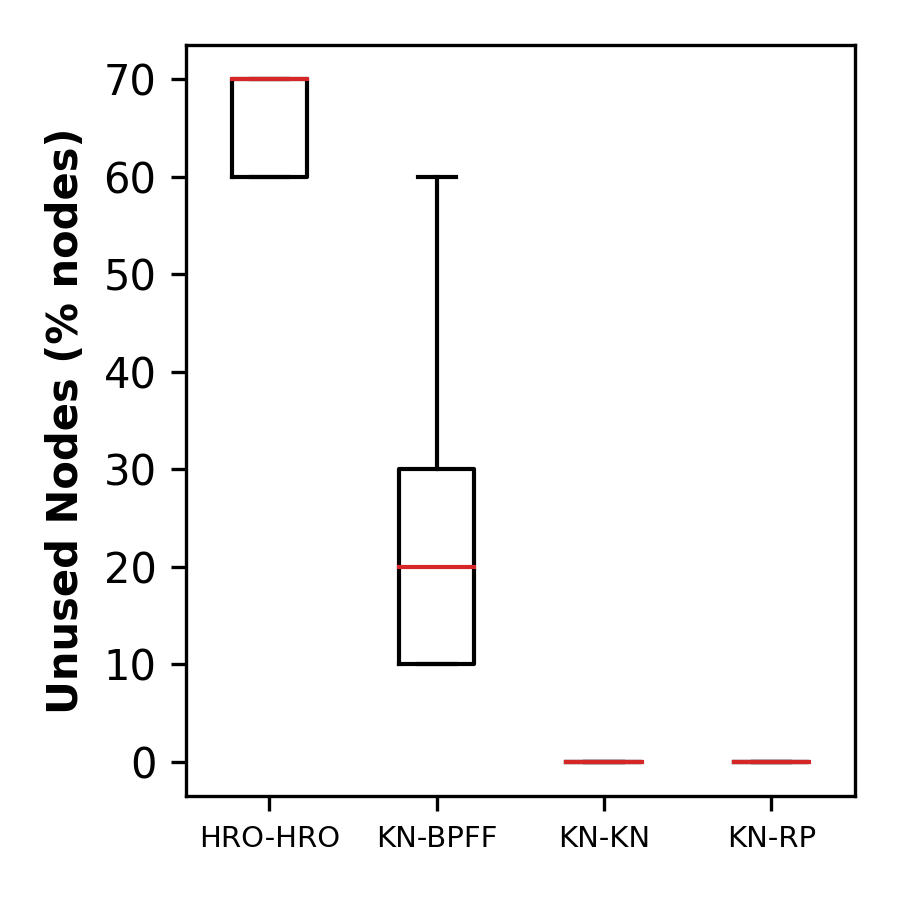
\includegraphics[width=0.28\linewidth]{4_Chapitre4/figures/evaluation/z-nodes-20221212-232143-169224.png}
    }\qquad
    \subfloat[QoS violations (based on tasks with missed deadline)\label{figure:herofake-evaluation-full-penalty}]{
        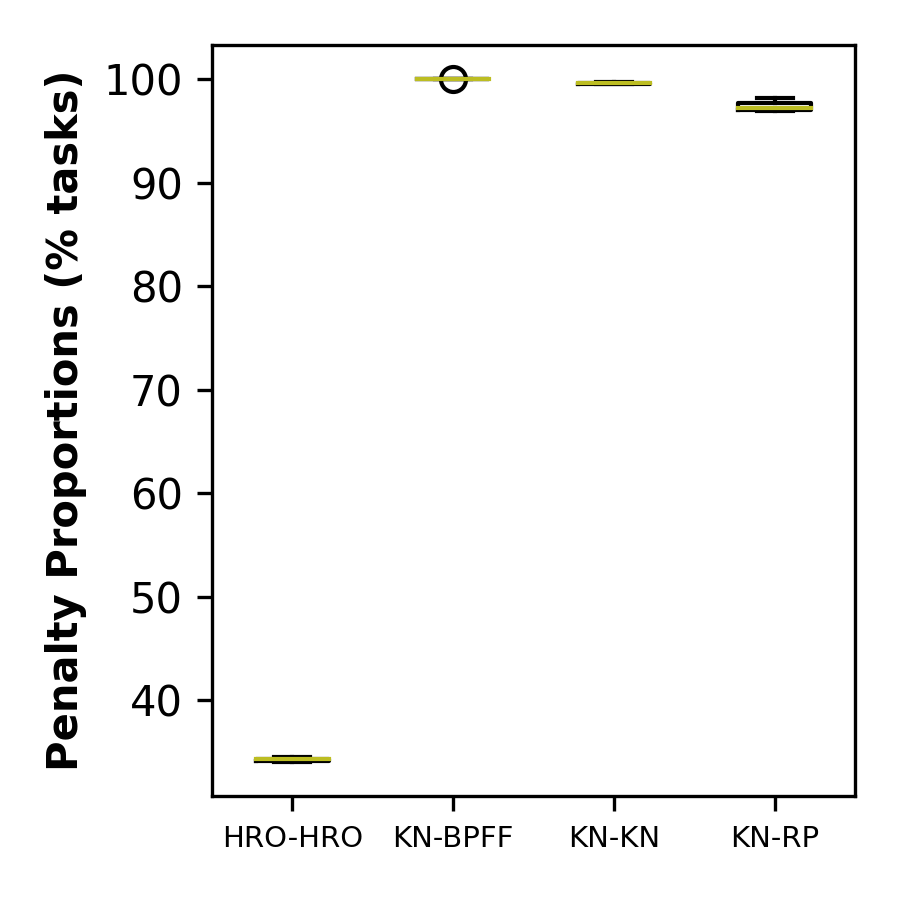
\includegraphics[width=0.28\linewidth]{4_Chapitre4/figures/evaluation/z-penalty-20221212-232143-169224.png}
    }\qquad
    \subfloat[Dynamic energy consumption (in kWh)\label{figure:herofake-evaluation-full-energy}]{
        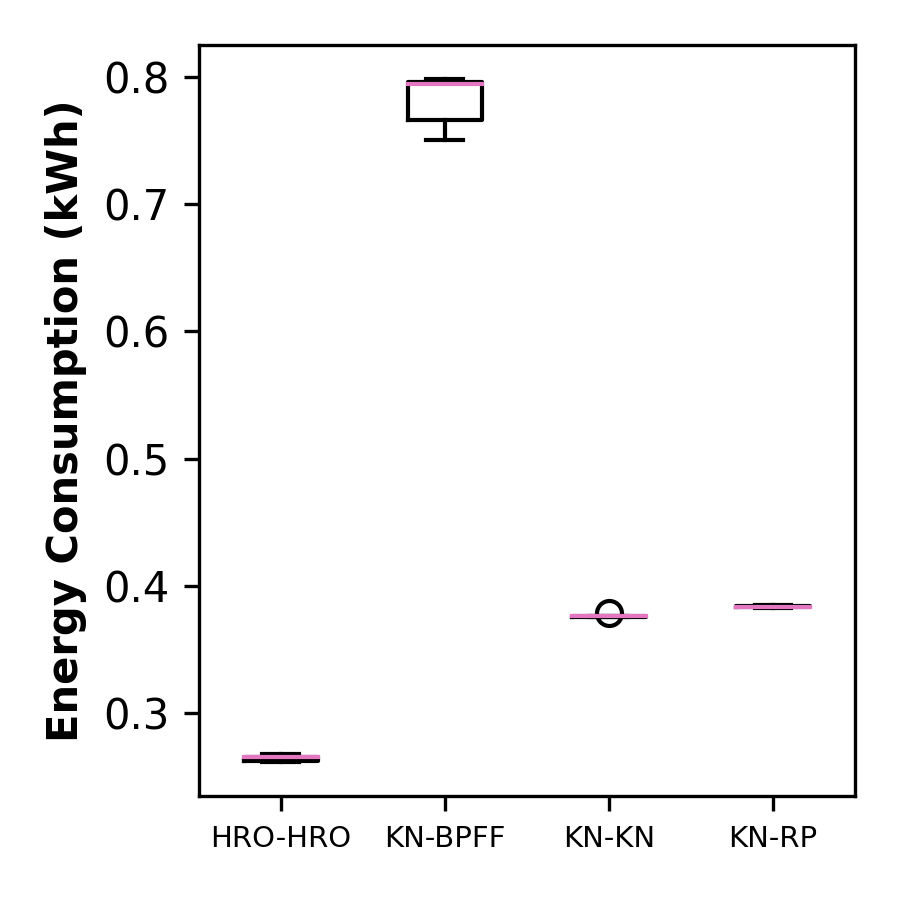
\includegraphics[width=0.28\linewidth]{4_Chapitre4/figures/evaluation/z-energy-20221212-232143-169224.png}
    }
    \caption{Evaluation 1 -- Comparison against baselines}
    \label{figure:herofake-evaluation-hro-full}
\end{figure*}

\begin{figure*}[!ht]
    \centering
    \subfloat[Task consolidation (based on the unused node count)\label{figure:herofake-evaluation-mixed-nodes}]{
        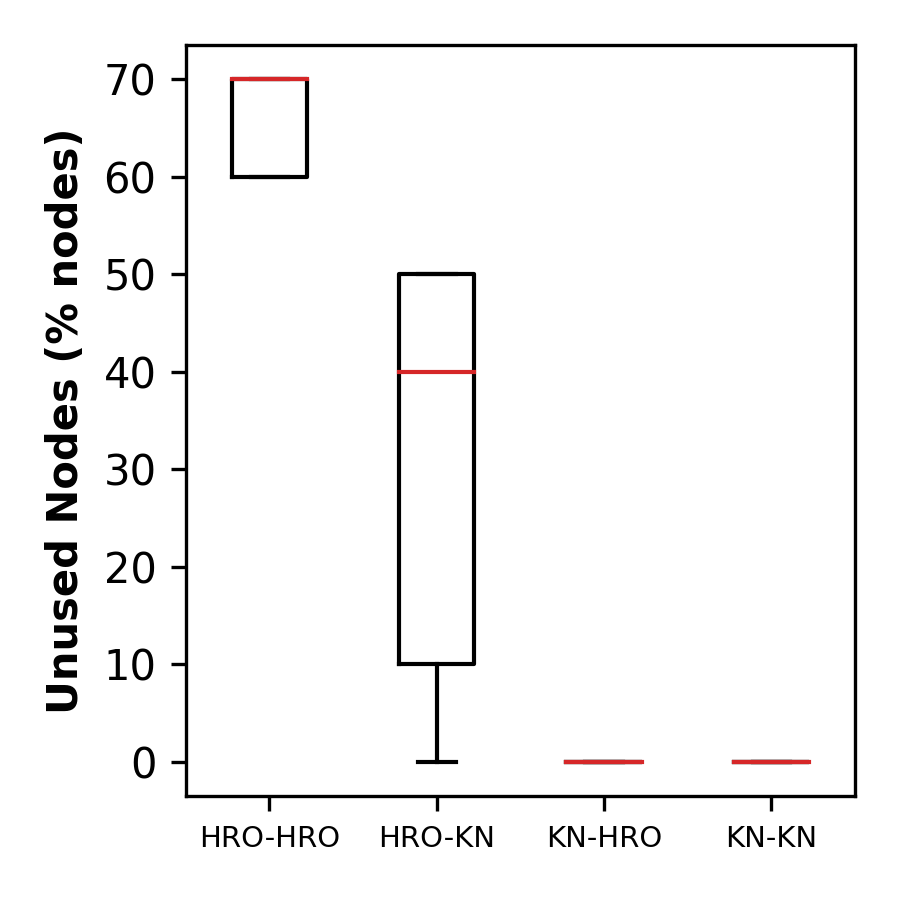
\includegraphics[width=0.28\linewidth]{4_Chapitre4/figures/evaluation/x-nodes-20221212-185844-053283.png}
    }\qquad
    \subfloat[QoS violations (based on tasks with missed deadline)\label{figure:herofake-evaluation-mixed-penalty}]{
        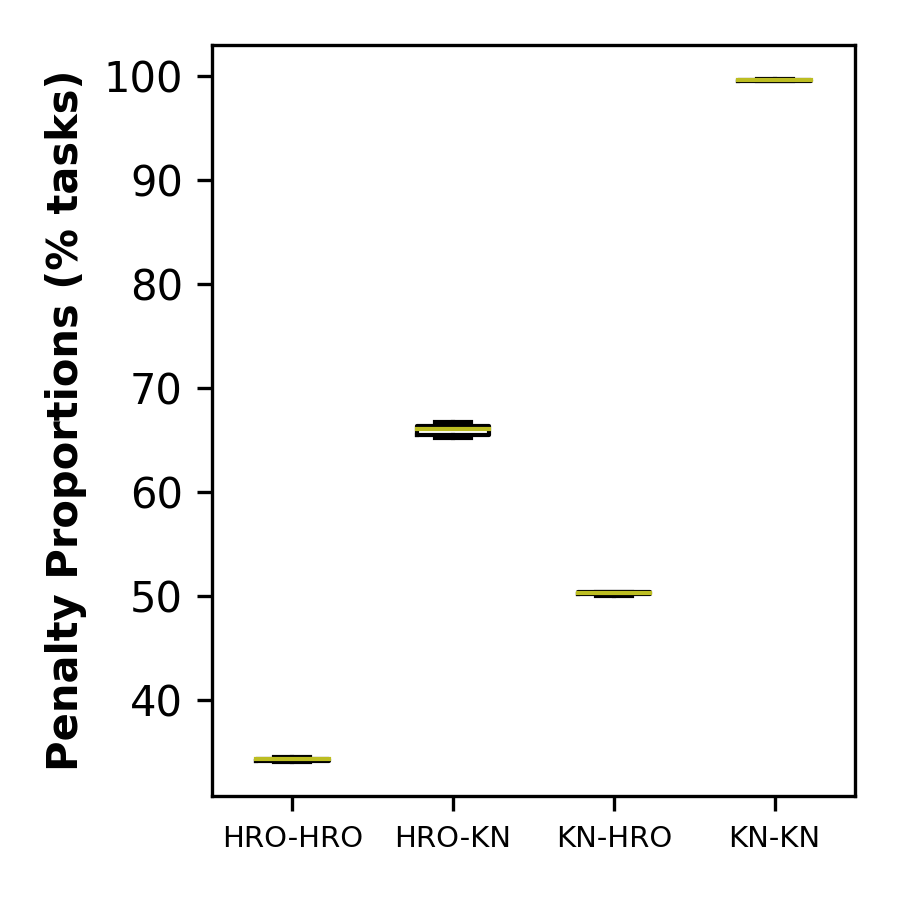
\includegraphics[width=0.28\linewidth]{4_Chapitre4/figures/evaluation/x-penalty-20221212-185844-053283.png}
    }\qquad
    \subfloat[Dynamic energy consumption (in kWh)\label{figure:herofake-evaluation-mixed-energy}]{
        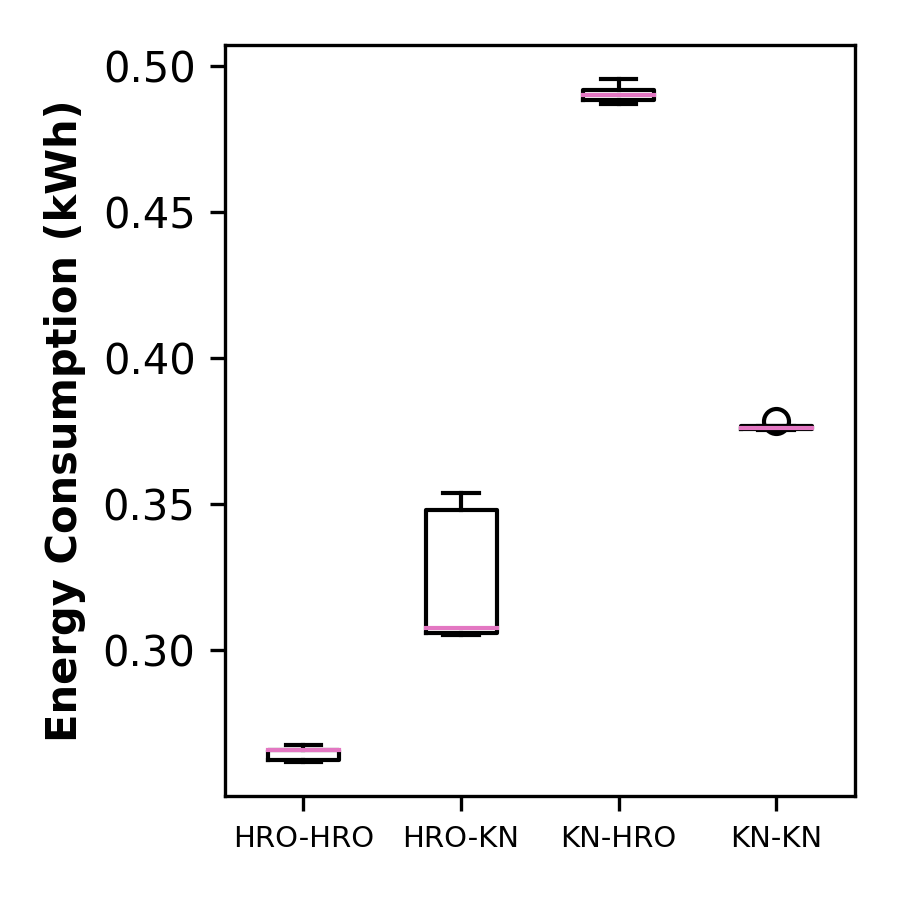
\includegraphics[width=0.28\linewidth]{4_Chapitre4/figures/evaluation/x-energy-20221212-185844-053283.png}
    }
    \caption{Evaluation 2 -- Impact of HeROfake components on the overall performance}
    \label{figure:herofake-evaluation-hro-mixed}
\end{figure*}

\subsection{Protocole expérimental}

Nous avons utilisé des mesures provenant de l'évaluation de trois modèles d'apprentissage différents (voir tableau~\ref{table:herofake-tasks}). Ces modèles ont été mis en œuvre sur trois plateformes d'exécution différentes (voir tableau~\ref{table:herofake-platforms}) comme expliqué dans la section~\ref{section:herofake-offline}.

Ces données ont servi en entrée à un simulateur que nous avons développé en utilisant la bibliothèque de simulation à évènements discrets SimPy~\cite{simpy}. Le simulateur suit le modèle décrit dans les sections~\ref{model:nodes}, \ref{model:platforms}, et \ref{model:tasks}.

Nous avons mesuré les délais de démarrage à froid pour les applications de notre étude de cas (tableau~\ref{table:herofake-tasks}). Il apparaît que les temps d'exécution pour les fonctions considérées sont dominés par les délais de démarrage à froid, ce qui fait de l'allocation adéquate des ressources une exigence stricte pour respecter les accords de niveau de service.

Dans la partie consacrée à l'évaluation des performances, nous comparons deux autoscalers :

\begin{itemize}
    \item HeROfake (HRO) -- Notre allocateur de ressources basé sur les métadonnées et conscient de l'hétérogénéité matérielle ;
    \item Knative (KN) -- Nous avons modélisé le comportement de l'autoscaler de Knative du mieux que nous avons pu, en nous appuyant sur la documentation disponible au moment de cette étude~\cite{knative-autoscaling}.
\end{itemize}

Notre évaluation comporte quatre ordonnanceurs :

\begin{itemize}
    \item HeROfake (HRO) -- Notre ordonnanceur conscient des coûts qui minimise les violations de SLA, la consommation d'énergie et la quantité totale de ressources engagées ;
    \item Knative (KN) -- Knative sélectionne une réplique sur le nœud le plus disponible~\cite{sureshENSUREEfficientScheduling2020}. Les répliques sont triées en fonction du nombre de requêtes en cours de traitement. La réplique avec la file d'attente la plus courte est sélectionnée ;
    \item Random Placement (RP) -- Les tâches sont assignées à une réplique aléatoire sur un nœud aléatoire ;
    \item Bin Packing First-Fit (BPFF) -- Les tâches sont consolidées sur un nombre minimum de répliques. L'ordonnanceur place les requêtes sur une première réplique jusqu'à ce que celle-ci atteigne son seuil de concurrence. BPFF est susceptible d'être la politique d'ordonnancement mise en œuvre pour AWS Lambda~\cite{wangPeekingCurtainsServerlessb}.
\end{itemize}

Nous avons conçu une évaluation des performances en deux étapes basée sur des simulations :

\begin{itemize}
    \item \textbf{Comparaison aux politiques de référence} (figure~\ref{figure:herofake-evaluation-hro-full}) : dans cette partie, nous avons comparé notre combinaison d'autoscaler et d'ordonnanceur, HeROfake (HRO-HRO), à : (1) l'autoscaler et l'ordonnanceur Knative complet (KN-KN), (2) l'autoscaler Knative avec l'ordonnanceur BPFF (KN-BPFF), (3) l'autoscaler Knative avec l'ordonnanceur RP (KN-RP) ;
    \item \textbf{Impact des composants sur la performance globale} (figure~\ref{figure:herofake-evaluation-hro-mixed}) : nous discutons ici de l'impact individuel de chacun des autoscalers et ordonnanceurs. Pour ce faire, nous avons conçu différentes stratégies : (1) en utilisant l'autoscaler HeROfake avec l'ordonnanceur Knative (HRO-KN), et (2) en utilisant l'autoscaler Knative avec l'ordonnanceur HeROfake (KN-HRO), puis nous avons comparé ces stratégies avec les versions complètes de HeROfake (HRO-HRO) et Knative (KN-KN).
\end{itemize}

La dénomination de chaque scénario dans ces figures se compose de deux parties séparées par un délimiteur. La première partie correspond à la politique d'allocation, la seconde à la politique d'ordonnancement (par exemple, HRO-KN signifie que nous avons utilisé l'autoscaler HeROfake en conjonction avec l'ordonnanceur Knative).

Pour chacune des combinaisons de politiques d'autoscaler et d'ordonnanceur, nous avons réalisé l'expérience sur la base d'un scénario à charge de travail synthétique, composée de 50000 tâches (requêtes utilisateur). Les tâches se voient attribuer un type aléatoire (ResNet50, VGG16 ou VGG19) et un niveau de QoS aléatoire (élevé, moyen, faible) suivant une distribution uniforme, avec des facteurs de ralentissement pour la QoS respectivement fixés à 2, 3 et 4. L'infrastructure du scénario se compose de 10 nœuds sur lesquels sont réparties 18 plateformes d'exécution (10 CPU, 6 GPU, 2 FPGA).

Les pondérations pour le niveau de concurrence (équation~\ref{eq:herofake-HRO-concurrency-target}) ont été fixées à $k_{ET} = \frac{2}{3}$, $k_{EC} = \frac{1,5}{6}$ et $k_{HP} = \frac{0,5}{6}$. Les pondérations pour la décision de mise à l'échelle (équation~\ref{eq:herofake-HRO-allocation-cost-function}) ont été fixées à $k_{TT} = \frac{2}{3}$, $k_{EC} = \frac{1,5}{6}$ et $k_{HP} = \frac{0,5}{6}$. Les pondérations pour la décision d'ordonnancement (équation~\ref{eq:herofake-HRO-scheduling-cost-function}) ont été fixées à $k_{QP} = \frac{2}{3}$, $k_{EC} = \frac{0,5}{6}$ et $k_{TC} = \frac{1,5}{6}$.

\subsection{Analyse des résultats}

\subsubsection{Comparaison aux politiques de référence}

\textbf{Consolidation des tâches}. La figure~\ref{figure:herofake-evaluation-full-nodes} montre que notre combinaison d'autoscaler et d'ordonnanceur permet d'obtenir le plus grand nombre de nœuds inutilisés. Avec l'autoscaler de Knative, l'ordonnanceur BPFF assure la meilleure consolidation, mais cette politique nécessite toujours plus de trois fois le nombre de nœuds que nous allouons avec notre politique.

\textbf{Accords de niveau de service}. La figure~\ref{figure:herofake-evaluation-full-penalty} montre que HRO-HRO est le plus performant en termes de violations de la QoS, avec 35\% de tâches qui ne respectent pas les délais. Il s'agit d'une amélioration considérable par rapport aux résultats de Knative, où les tâches ne respectent pas leur échéance dans plus de 99\% des cas : le retard introduit par l'allocation réactive des ressources ne peut pas être compensé à temps en utilisant uniquement des CPU.

\textbf{Consommation d'énergie}. La figure~\ref{figure:herofake-evaluation-full-energy} montre que notre politique, avec l'autoscaler et l'ordonnanceur HRO fonctionnant conjointement, est toujours la plus performante en termes de consommation d'énergie dynamique. Cela s'explique évidemment par le fait que nous allouons des accélérateurs matériels ; cependant, au cours de notre évaluation, la durée d'exécution de notre scénario est similaire avec les politiques Knative et HRO (environ 13,5 minutes). La politique d'ordonnancement BPFF est également la moins performante en termes de temps d'exécution, car elle maximise la taille des files d'attente dans les répliques, ce qui donne les pires résultats en termes de consommation d'énergie.

\subsubsection{Impact des composants individuels}

\textbf{Consolidation des tâches}. La figure~\ref{figure:herofake-evaluation-mixed-nodes} montre que HRO-HRO est le plus performant en matière de consolidation des tâches, laissant un peu moins de 70\% des nœuds disponibles inutilisés, alors que l'ordonnanceur de Knative, dans le framework de notre politique d'autoscaling, n'atteint que 40\% de nœuds inutilisés. Ce résultat est attendu, car l'ordonnanceur de Knative utilise une politique de répartition de charge. Les résultats de consolidation de KN-HRO sont médiocres, mais pour une raison différente : notre ordonnanceur tente de minimiser les violations de la qualité de service en répartissant la charge sur tous les processeurs alloués.

\textbf{Accords de niveau de service}. La figure~\ref{figure:herofake-evaluation-mixed-penalty} montre que notre ordonnanceur ne fonctionne pas bien en conjonction avec l'autoscaler de Knative. En effet, notre ordonnanceur tente de minimiser les pénalités : lorsqu'il ne dispose que de CPU, il se comporte de la même manière que l'ordonnanceur de Knative et répartit les tâches sur ces CPU afin de limiter les violations de qualité de service. Cependant, notre ordonnanceur sous l'autoscaler Knative parvient toujours à maintenir les violations de la qualité de service à environ 50\% des tâches, ce qui montre qu'il y a une marge d'amélioration même lorsque les tâches d'inférence sont déployées sur des CPU uniquement, en jouant sur la politique de sélection des requêtes. On note que lors de notre évaluation, l'autoscaler Knative a donné les pires résultats en ce qui concerne la fréquence des démarrages à froid (6,5 fois plus fréquents avec KN-HRO qu'avec HRO-KN).

\textbf{Consommation d'énergie}. La figure~\ref{figure:herofake-evaluation-mixed-energy} montre que la consommation d'énergie est toujours plus faible lorsque l'on utilise notre autoscaler, qui peut allouer des accélérateurs matériels. En revanche, notre ordonnanceur utilisé avec l'autoscaler de Knative donne les pires résultats en termes de consommation d'énergie. Cela s'explique à nouveau par le fait que l'ordonnanceur tente de minimiser les pénalités en répartissant les tâches sur un grand nombre de CPU, la plateforme d'exécution la plus consommatrice en énergie dans notre cas d'étude.

\section{Travaux connexes}
\label{section:herofake-sota}

Plusieurs contributions antérieures se sont concentrées sur les plateformes de mise à l'échelle automatique pour le déploiement de tâches de courte durée, comprises dans des applications présentant des motifs d'utilisation imprévisibles. Le tableau~\ref{table:herofake-sota} résume les différences entre ces contributions et notre plateforme cible.

Certaines de ces contributions ont tenté d'atteindre les SLA avec des ressources non réservées~\cite{gujaratiSwayamDistributedAutoscaling2017, zhangMArkExploitingCloud, mampageDeadlineawareDynamicResource2021, singhviAtollScalableLowLatency2021, handaoui2020releaser, handaoui2020salamander, yalles2022riscless}. Parmi ces contributions, certaines se concentrent sur l'utilisation de ressources matérielles hétérogènes supplémentaires pour accélérer l'exécution de la charge de travail~\cite{zhangMArkExploitingCloud, lingPigeonDynamicEfficient2019, yangINFlessNativeServerless2022}. Ces méthodes nécessitent souvent un surprovisionnement des ressources pour utiliser l'accélération matérielle, par exemple en s'appuyant sur des instances AWS dans le cloud public qui donnent accès à des GPU~\cite{zhangMArkExploitingCloud}, en utilisant un pool de conteneurs préchauffés~\cite{lingPigeonDynamicEfficient2019}, ou même en provisionnant de manière proactive des nœuds pour respecter des échéances définies par l'utilisateur~\cite{singhviAtollScalableLowLatency2021}. Ces solutions, bien qu'intéressantes, peuvent toutefois s'avérer insuffisantes en termes d'usage des ressources et entraîneraient une consommation d'énergie supplémentaire dans un cloud privé.

En outre, certains auteurs se concentrent sur des infrastructures homogènes \cite{gujaratiSwayamDistributedAutoscaling2017, sureshENSUREEfficientScheduling2020, mampageDeadlineawareDynamicResource2021, singhviAtollScalableLowLatency2021, yangINFlessNativeServerless2022}. Ces études pourraient difficilement s'adapter au contexte du cloud privé que nous visons, où les ressources sont généralement éphémères et hétérogènes. En outre, certaines de ces contributions proposent des modèles de tâches qui ne couvrent pas la possibilité d'accords de niveau de service définis par l'utilisateur et à la granularité d'une requête~\cite{sureshENSUREEfficientScheduling2020, lingPigeonDynamicEfficient2019}. Enfin, certaines de ces contributions sont axées sur les performances plutôt que sur les coûts, ce qui est crucial dans notre contexte de cloud privé~\cite{gujaratiSwayamDistributedAutoscaling2017, lingPigeonDynamicEfficient2019, singhviAtollScalableLowLatency2021, choSLADrivenMLInference}.

Bien que la consommation d'énergie soit l'un des éléments les plus importants du coût total d'exploitation (\textit{OPEX}, pour \textit{Operational Expenditure}) dans un centre de données -- dépassant parfois le coût d'achat du matériel~\cite{7279063}, à notre connaissance, aucune de ces contributions ne couvre l'impact de l'allocation et du placement dynamiques sur la consommation d'énergie, ni ne considère la consommation d'énergie comme une métrique de qualité de service. Il s'agit d'une limitation sérieuse, car l'optimisation de la consolidation des tâches ouvre la voie à des politiques de ralentissement et de mise hors tension qui peuvent avoir un impact positif majeur sur l'efficacité énergétique d'un centre de données~\cite{chaurasiaComprehensiveSurveyEnergyaware2021}.

\section{Conclusion et perspectives}
\label{section:herofake-conclusion}

Dans ce chapitre, nous avons présenté HeROfake, notre framework pour le déploiement de tâches de détection de deepfake, basées sur des fonctions interactives et de courte durée, sur un cloud privé hétérogène dans le modèle serverless.

Nous avons présenté les deux phases qui composent ce framework : une phase hors-ligne au cours de laquelle nous caractérisons les performances des plateformes d'exécution et les exigences des fonctions ; et une phase en ligne au cours de laquelle nous allouons dynamiquement les ressources et ordonnançons les tâches à exécuter sur ces plateformes.

Les résultats expérimentaux montrent que si le temps total d'exécution des tâches sous HeROfake est similaire à celui de Knative, nous obtenons une réduction de plus de 60\% des pénalités de qualité de service ; les tâches sont consolidées sur moins de 40\% des nœuds de l'infrastructure, 77\% des plateformes d'exécution restant inutilisées ; enfin, la consommation d'énergie dynamique est réduite de 35\% par rapport à Knative.

L'inclusion du traitement vidéo dans le framework est un défi intéressant, car il introduirait des dépendances entre les tâches. Les exécutions de fonctions ne seraient plus \textit{sans état}, ce qui entraînerait la nécessité de s'intéresser au problème du stockage des données intermédiaires dans une infrastructure serverless.

Nous avons également l'intention d'étendre notre cadre d'étude en se donnant la possibilité d'utiliser des traces d'exécution réelles comme scénarios d'entrée, au lieu de générer uniquement des charges de travail synthétiques.
